\documentclass{article}
\usepackage[english]{babel}

% Set page size and margins
% Replace `letterpaper' with `a4paper' for UK/EU standard size
\usepackage[letterpaper,top=2cm,bottom=2cm,left=3cm,right=3cm,marginparwidth=1.75cm]{geometry}

% Useful packages
\usepackage{amsmath}
\usepackage{graphicx}
\usepackage[colorlinks=true, allcolors=blue]{hyperref}
\usepackage{longtable}
\usepackage[round]{natbib}

\begin{document}
\begin{titlepage} 
    \title{}
    \centering 
    \vspace*{1in} 
    \begin{Large}\bfseries 
    Identifying Inconsistencies in Data Quality Between FAOSTAT, WOAH, UN Agriculture Census, and National Data\par 

    \vspace{2in} 
    Ian McKechnie \href{mailto:imckechn@uoguelph.ca}{imckechn@uoguelph.ca}

    Kassy Raymond \href{mailto:kraymond@uoguelph.ca}{kraymond@uoguelph.ca}

    Dr. Deborah Stacey \href{mailto:dastacey@uoguelph.ca}{dastacey@uoguelph.ca}

    \vspace{3in} 
    The Global Burden of Animal Diseases
    
    \end{Large} 
    \vspace{1.5in} 
    \vfill 
    \par 
    
    % \author{Ian McKechnie \\ email \href{mailto:imckechn@uoguelph.ca}{imckechn@uoguelph.ca} 
    %     \and Kassy Raymond \\ email \href{mailto:kraymond@uoguelph.ca}{kraymond@uoguelph.ca} 
    %     \and Dr. Deborah Stacey \\ email \href{mailto:dastacey@uoguelph.ca}{dastacey@uoguelph.ca}}

    % \date{\parbox{\linewidth}{\centering%
    %       \today\endgraf\bigskip
    %       The Global Burden of Animal Diseases Informatics }}
    % \par 
    % \maketitle
    % \vspace{0.5in} 
    % September 2023 
    \par 
\end{titlepage} 

% \begin{titlepage}
%     \begin{center}
%     \vspace*{1cm}
%     \title{}

%     \vspace{20cm}
%     \author{Ian McKechnie \\ email \href{mailto:imckechn@uoguelph.ca}{imckechn@uoguelph.ca} 
%         \and Kassy Raymond \\ email \href{mailto:kraymond@uoguelph.ca}{kraymond@uoguelph.ca} 
%         \and Dr. Deborah Stacey \\ email \href{mailto:dastacey@uoguelph.ca}{dastacey@uoguelph.ca}}

%     \date{\parbox{\linewidth}{\centering%
%           \today\endgraf\bigskip
%           The Global Burden of Animal Diseases Informatics }}

%     \maketitle

%     \end{center}
% \end{titlepage} 



\begin{abstract}
With the growth of AI and data modelling, the old saying by George Fuechsel regarding data quality ‘Garbage in, garbage out’ holds more truth than ever. Data Scientists are learning the quality of their models depends on the quality of data. Data used by the Global Burden of Animal Diseases (GBADs) is available to modellers around the world and the quality of the data provided is important as it is used in modelling disease, greenhouse gas emissions, and more. These are important topics so the data given to the modellers must be investigated and checked for internal and external inconsistencies. The goal of this paper is to investigate data provided by GBADs to find inconsistencies in the data. Data quality was analyzed using a five-year trailing average comparison, the interquartile range for the yearly rates of change, and observing outliers on a normal distribution for the yearly rates of change for livestock populations over time. 
The normal distribution and interquartile range analysis is an internal data analysis that can find outliers that indicate possible data inconsistencies. The five-year trailing average helps identify external data inconsistencies between sources. Using purpose-built data analysis tools and performing analysis on the data shows there are inconsistencies in the data. The consequences of these findings show that researchers need to be cognizant of the data they are using and need to perform their own analysis before they use it in their models as the results can show incorrect results.
\newline
\newline
Key Words: Data Science, Modelling, Data Quality, AI

\end{abstract}

\section{Introduction}

Livestock population data measured on a national and sub-national level are important statistics in the calculation of animal disease \citep{sibhat_bovine_2017}, economic health burden \citep{muraguri_cost_1998}, climate change \citep{geoffry_fordyce_australian_nodate}, and antimicrobial resistance calculations \citep{mulchandani_global_2023}. Analysis performed using data for these purposes should be as accurate and complete as possible so models using this data can have optimal predictions. The accuracy and completeness of the data \citep{penell_validation_2008} are measured based on what can be estimated as the population of the animals. Since these data sources acquire their data by surveying the population \citep{world_organization_for_animal_health_world_nodate}, it can be hard to know the exact animal population at any time \citep{world_organization_for_animal_health_world_nodate}. Currently, livestock population data is reported by the Food and Agriculture Organization Corporate Statistical Database (FAOSTAT), the World Organization for Animal Health (WOAH), United Nations Census reports, and national statistics agencies (NSAs). GBADs provides the FAOSTAT and WOAH data through their publicly accessible API. The Census \cite{WorldCensusOne} \cite{WorldCensusTwo} and national data \cite{USDA} were acquired for this paper. Despite all sources being reputable, the data varies widely between them, and an individual source of data is subject to inconsistencies or inaccuracies. Therefore, it is important to bring awareness of these inconsistencies to researchers who use these data for their modelling and calculations. 

The objective of this paper is to investigate discrepancies between the sources and individual source inconsistencies using three different approaches. These approaches have been chosen to visualize and quantify data differences for multiple species and countries. Each approach considered a different aspect of data quality to achieve the following: 

\begin{enumerate}
\item To identify yearly rates of change that are highly improbable,
\item To determine whether the interquartile range (IQR) can be used to identify outliers in three data sources, and
\item To determine a trailing five-year population average to visualize high-level data trends.
\end{enumerate}

One reason why data is different between FAOSTAT and WOAH is because of how they are sampled. FAOSTAT uses different sources such as national statistical offices, ministries of agriculture, and other governmental organizations \citep{faostat_data_nodate} to get the populations of livestock in each country \citep{world_organization_for_animal_health_world_nodate}. WOAH gathers data from its member countries by collaborating with veterinary authorities and laboratories \citep{world_organization_for_animal_health_world_nodate}. What makes these two approaches for data collection different is how the sources get their data, either by recording it through observation or by sending out surveys. This often results in slightly different data for the same country. To understand more about how complicated surveying data is, see section 4.2.2.

\section{Background}
Previous work by \cite{faye_how_2020}  and \cite{geoffry_fordyce_australian_nodate} investigated the quality of livestock census data in camelids and cattle, respectively.  Both studies noted that data quality may be impacted by difficulties tracking nomadic people and animals and that people may be dishonest in government surveys to avoid paying higher taxes, leading to inaccurate or incorrect data. We build upon the analyses of \cite{faye_how_2020} and \cite{geoffry_fordyce_australian_nodate} by investigating inconsistencies through creating and analyzing data visualizations and identifying ranges in the data that exhibit irregularities or possible inaccuracies. 

The methods used for data analysis have been used in the past for data analysis because they can show outliers with relative ease \citep{oracle_outlier_nodate}. For the first method which is the yearly rate of change, when plotting all of the yearly population rate of change data points it will make a normal curve. It is known in statistics that any data outside plus or minus three standard deviations of the median is considered an outlier \citep{oracle_outlier_nodate}. For the IQR, it is also true that this is an established method to discover outliers \citep{Vinutha2018DetectionOO}. The only difference between this and the other methods for finding outliers is that extreme outliers can influence the upper and lower fence placement \citep{oracle_outlier_nodate} so it needs to be noted when using the IQR for analysis that the user tries removing extreme outliers to observe how it affects the upper and lower fences to then possibly investigate any new data points that exist beyond the fences. The final approach taken in this work is the trailing five-year average where averages are plotted as a histogram and inconsistencies are identified by humans. This method of analysis is typically used in stock price analysis \citep{law_insider_five_nodate} but can be used for other forms of analysis as well. The reason it is used here is because it shows macro trends and can help spot general points of time when population trajectories changed. This is a manual process that can show the user a general time frame to investigate to get a better understanding of what was going on at that time to influence the population. 

These methods used are not limited to comparing population data, they can be used for comparing other data as long as it's from multiple sources and the data is of the same subject. These methods compare multiple sources and identify areas that have the largest variation between the two sources. This can be useful for almost any topic such as population estimates of people, agriculture production estimates, or economic activity estimates. Given that these are important topics and multiple sources track these, the statistical tools could help identify which source is more reliable over which periods of time.

Since the chosen methods show internal and external data inconsistencies, other methods for finding inconsistencies will find similar results, possibly including or excluding a few more points depending on what they define the inconsistency cut-off range to be. The reason these three were selected is because they minimize single-year impacts on the data being investigated and look for larger trends in the data.

This also limits the statistical methods and sources used. The limits of the statistical methods are that they outline time periods, but don't give much more information other than the date range and a measurement. It cannot tell us the different reasons why this happened. It is up to the researcher and that can be time-consuming. The sources also have their limits. There are known and unknown biases in the sources collected. WOAH and FAOSTAT do not collect their data and instead hire government and non-government agencies to collect the data on their behalf in their respective countries. These agencies could have their own biases or shortcomings not shown in the data. An agency could have biases that FAOSTAT or WOAH aren't even aware of that could skew the data to show a larger or smaller population than the true amount and researchers would not be able to find out.

\section{Methodology}
\subsection{Data collection and inclusion criteria }
Livestock population data from FAOSTAT and WOAH was obtained from the GBADs Application Programming Interface (API). This data was collected from the source by the GBADs Informatics team, but the original values and flags have been preserved. 

Data from agricultural censuses and surveys was also used in this analysis. Census data was obtained from the 2000 and 2010 World Census of Agriculture reports from the Food and Agriculture Organization of the United Nations \citep{WorldCensusOne, WorldCensusTwo}. The `2000 World Census of Agriculture' report contains census data from participating countries between 1996-2005 and the `2010 World Census of Agriculture' report contains the census data for participating countries between 2006-2015. 

The countries taken from these reports for our analysis were selected to have varying socioeconomic levels, population and land sizes, geolocations, and farming techniques. This was done to show that inconsistencies are not limited to a specific subset of countries. The countries studied are

Argentina, Australia, Botswana, Brazil, Canada, Chile, China, Egypt, Ethiopia, India, Indonesia, Ireland, Japan, Mexico, New Zealand

\subsection{Statistical methods for the identification of inconsistencies}
The objective of this paper is to find inconsistencies internally and externally in the data. To identify internal data inconsistencies, outliers need to be found when compared to data from that same source\citep{FasterCapital}. Here, we define and identify outliers using two methods; (1) plotting the yearly rates of change on a normal curve and finding outliers past three standard deviations, and (2) using a box plot to find the IQR for the yearly rates of change, and identify outliers. These methods will identify outliers thus allowing further analysis into these points to understand if the data is consistent or inconsistent. 

External inconsistencies are when a source’s data is very different than that of other sources \citep{lyles_validation_2011}. For this analysis, a direct comparison needs to be made between sources. Finding a trailing five-year average for the population of livestock for each half-decade for each source will be used to compare the sources to each other. This method reduces the effects of short-term change and shows general trends. The advantage of this method is that the graph can be analyzed to find long-term trends that do not match between sources which enables a future analysis to determine if the data is consistent or not between sources.

\section{Results}
The data from these four sources shows the animal population numbers for different countries. Since the sources claim to represent the population of livestock to the best of their abilities, the numbers should be similar across sources. The differences that will affect the populations between each source are the different data collection methods including different times when the population numbers were collected, different estimation techniques, and reporting pipelines between the sources and agencies. This results in the data not being complete (e.g. missing years), there being a large or impossible variance for a population between two consecutive years, or data from two sources greatly contradict each other. An example of internally and externally consistent data is in Figure~\ref{fig:image1} which shows that the cattle numbers in the USA reported by FAOSTAT, WOAH, the UN Agricultural Census, and USA national data are the same or similar for most years. 

%First Image
\begin{figure}[h!]
    \centering
    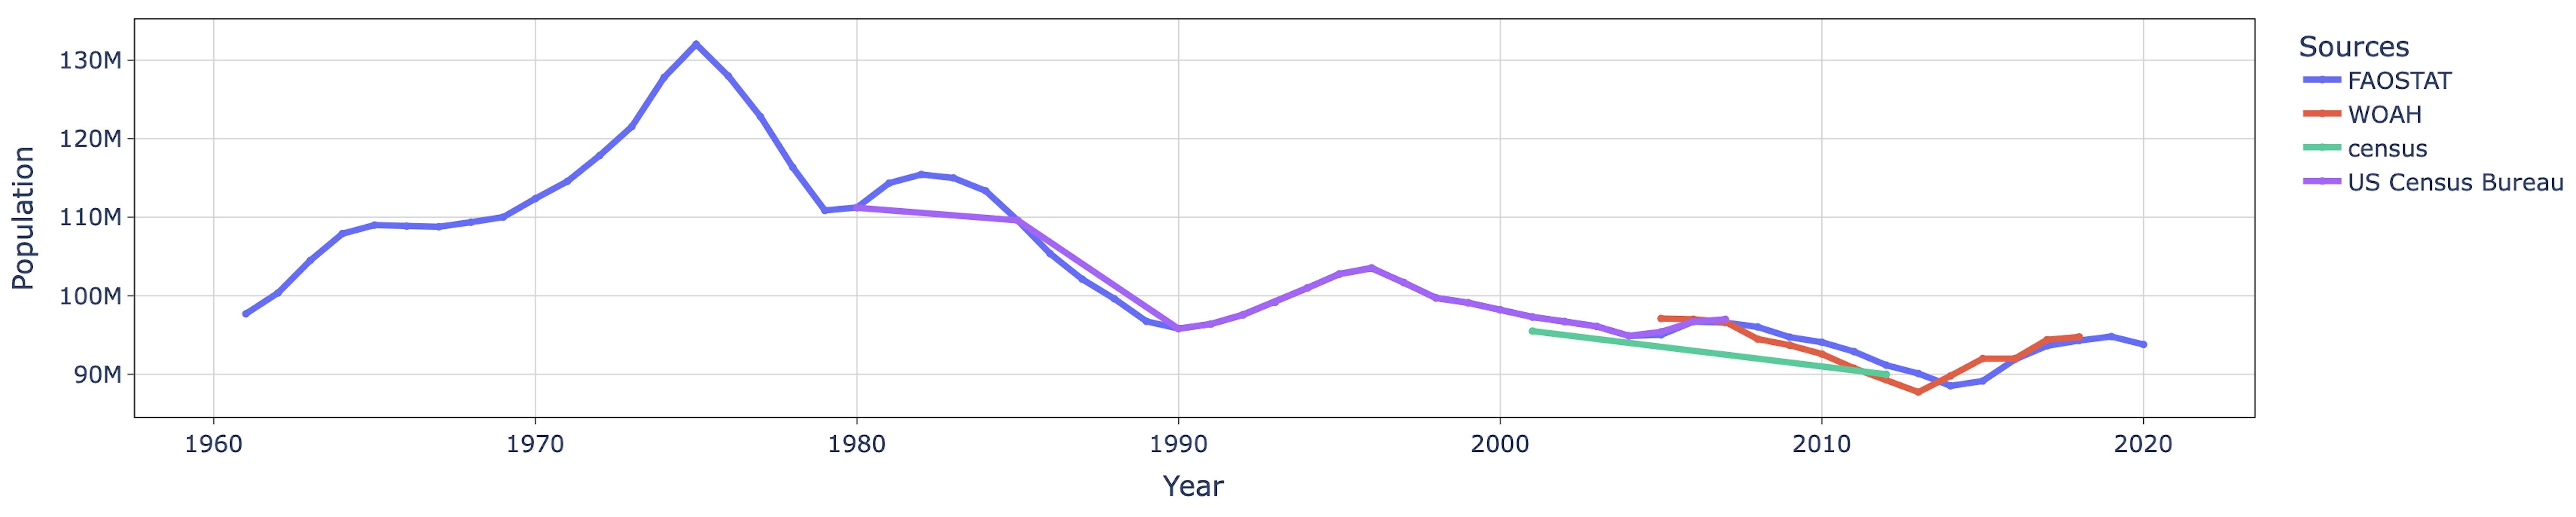
\includegraphics[width=1\textwidth]{image1}
    \caption{Graph of cattle Populations in the USA between 1960-2020}
    \label{fig:image1}
\end{figure}

An example of greater data inconsistency is shown in Figure ~\ref{fig:image2}. The number of sheep FAOSTAT reported in Ethiopia in 2009 is almost 60\% larger, roughly 10 million sheep, than WOAH for the same year. This could not be a simple rounding error. Another possible issue is that WOAH shows an almost 50 percent drop in sheep numbers between 2008 and 2009, and then a 51 percent increase between 2009 and 2011. FAOSTAT in comparison shows a steadily increasing animal population over those years with some slight variation in population numbers but nothing that varies as much as WOAH. This does not mean that FAOSTAT is automatically the 'better' source but it does raise issues with the collection of population numbers in this time period. Ethiopia has suffered several severe droughts and this may be impacting the livestock population numbers so it is necessary to investigate if the numbers in FAOSTAT (that are flagged as official numbers from Ethiopian sources) are accurate and if there was no drought effect on sheep numbers \citep{bogale_drought_2022}.

%Image two
\begin{figure}[h!]
    \centering
    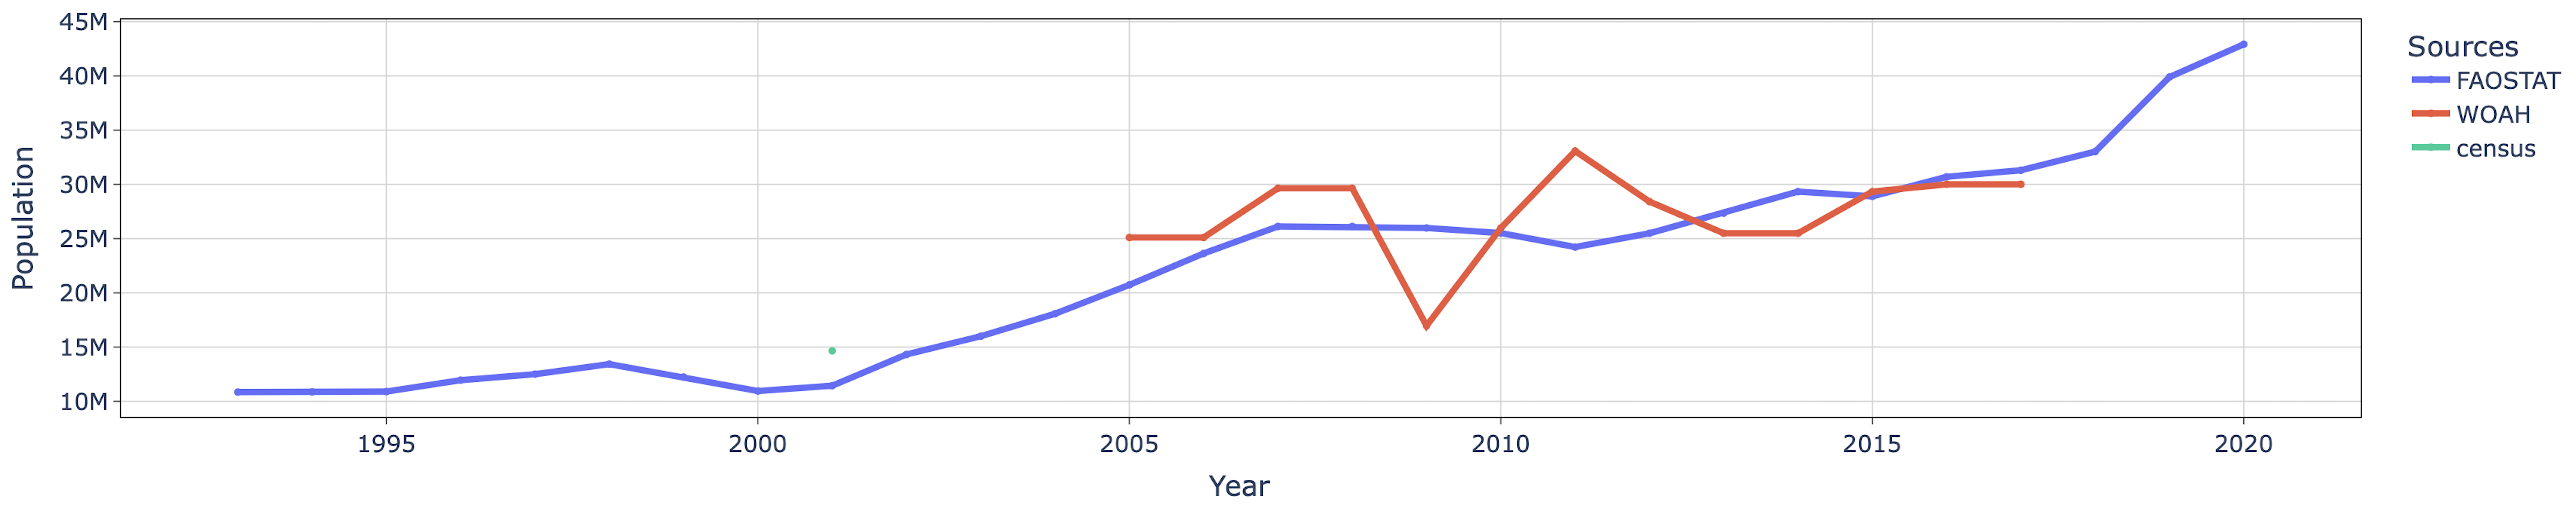
\includegraphics[width=1\textwidth]{image2}
    \caption{Graph of Sheep Populations in Ethiopia between 1993-2017}
    \label{fig:image2}
\end{figure}


Having viewed these large discrepancies in the animal population numbers between each source, it is clear there exists both external and internal inconsistencies in the population data examined. The following sections show three methods of visualizing and quantifying the difference in population numbers between all four sources. 

\subsection{Methods}
\subsubsection{Method 1: Normal Distribution of growth rates}
The first investigation was to identify yearly rates of change that are highly improbable (or need 'ground truth' verification from expert or in-country sources). To achieve this, we took all of the yearly growth rates for the population of animals in a country and then plotted them to produce a histogram overlaid with the normal curve.
Growth rates should have minimal variation between each other so most yearly growth rates should have similar magnitude and more unusual growth rates will appear less often. Performing analysis with a normal curve is done because animal populations should be relatively similar each year since animal populations typically have a sustainable growth rate unless perturbed by special circumstances (natural disasters, climate change, changing agricultural/economic policies, conflict). Each yearly growth rate will fit onto this normal curve and should be similar to past growth rates \citep{Pardoe_Simon_Young}. Normal distributions can also display standard deviations which is desirable because data points outside of the third standard deviation are generally considered to be outliers.

Using the normal curve, points outside three standard deviations can be labeled as outliers and it can be concluded that there is a high chance that they are internally inconsistent \citep{oracle_outlier_nodate}. This means that any year that the animal populations grew or shrank too quickly was most likely a suspicious data point that needed investigation and annotation for users of the data. This method is to compare yearly growths for a single data source at a time. For example, Figure~\ref{fig:image4} shows three standard deviations in either direction of the rates of change for the data shown in Figure~\ref{fig:image1}. The blue vertical line is the mean growth rate, the others being standard deviations. It is evident from the example that there are no data points outside the third  standard deviation indicating there are no outliers in this data. 

%Image Three
\begin{figure}[h!]
    \centering
    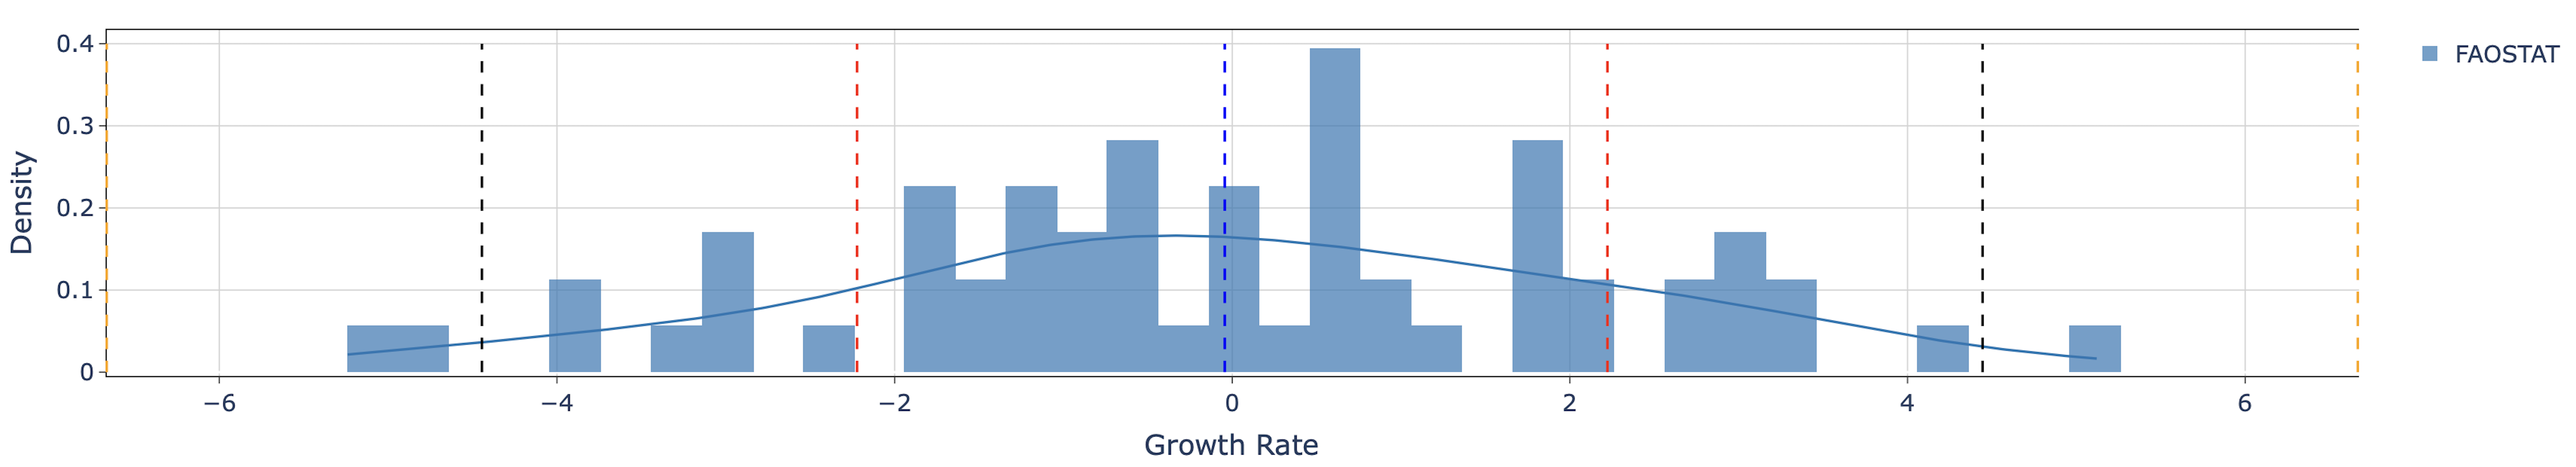
\includegraphics[width=1\textwidth]{image3}
    \caption{The growth rates for cattle in the USA from FAOSTAT are shown as a histogram with the normal curve superimposed on top. The first STD line is red, the second STD is black, and the third STD is yellow.}
    \label{fig:image3}
\end{figure}


%Image Four
\begin{figure}[h!]
    \centering
    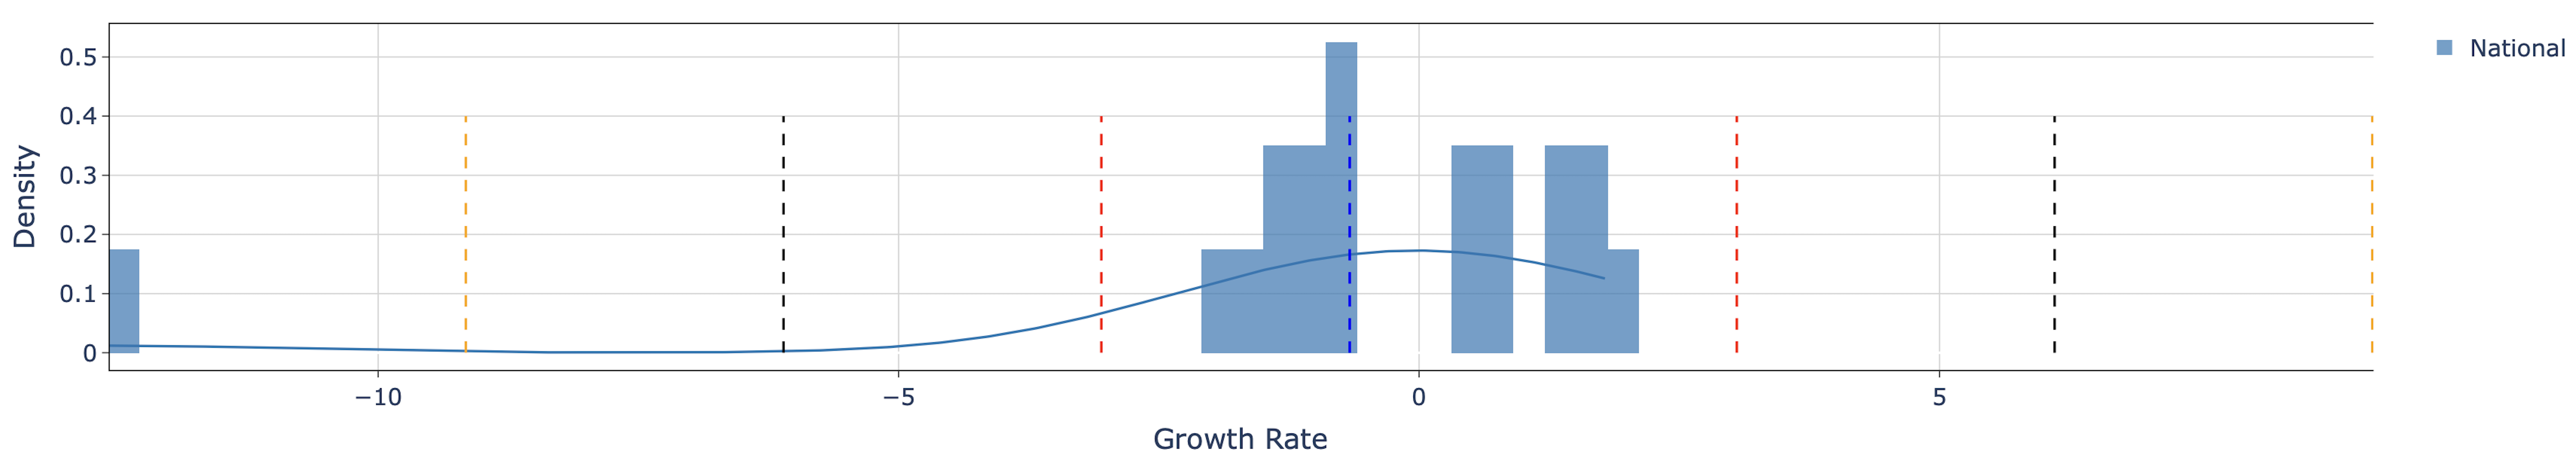
\includegraphics[width=1\textwidth]{image4}
    \caption{The growth rates for cattle in the USA from USA national data are shown as a histogram with the normal curve superimposed on top. The first STD line is red, the second STD is black, and the third STD is yellow.}
    \label{fig:image4}
\end{figure}

Inconsistencies were found in the FAOSTAT data as elucidated by Figure~\ref{fig:image2}. When looking at the growth rates for sheep in Ethiopia (Figure~\ref{fig:image2}) between 2008 and 2011 the graph has more higher positive and lower negative slopes. When looking at the rates of change for this in Figure~\ref{fig:image5} it can be seen that there is an outlier during this period. Over the same range, the rates of change for the WOAH data do not have an outlier at this point, indicating both FAOSTAT and WOAH have possible issues with data for this year. WOAH has consistency issues for data on Sheep in Ethiopia as well. All of WOAH's data falls between the third standard deviation lines but the third standard deviation exists at more than 40 percent growth. This shows the data changing rapidly each year. This is evidence that WOAH data is problematic for Sheep in Ethiopia. Once again, this does not immediately indicate that the WOAH numbers should be ignored by users, but they should be annotated and investigated (if possible).

% Images five and six
\begin{figure}[h!]
    \centering
    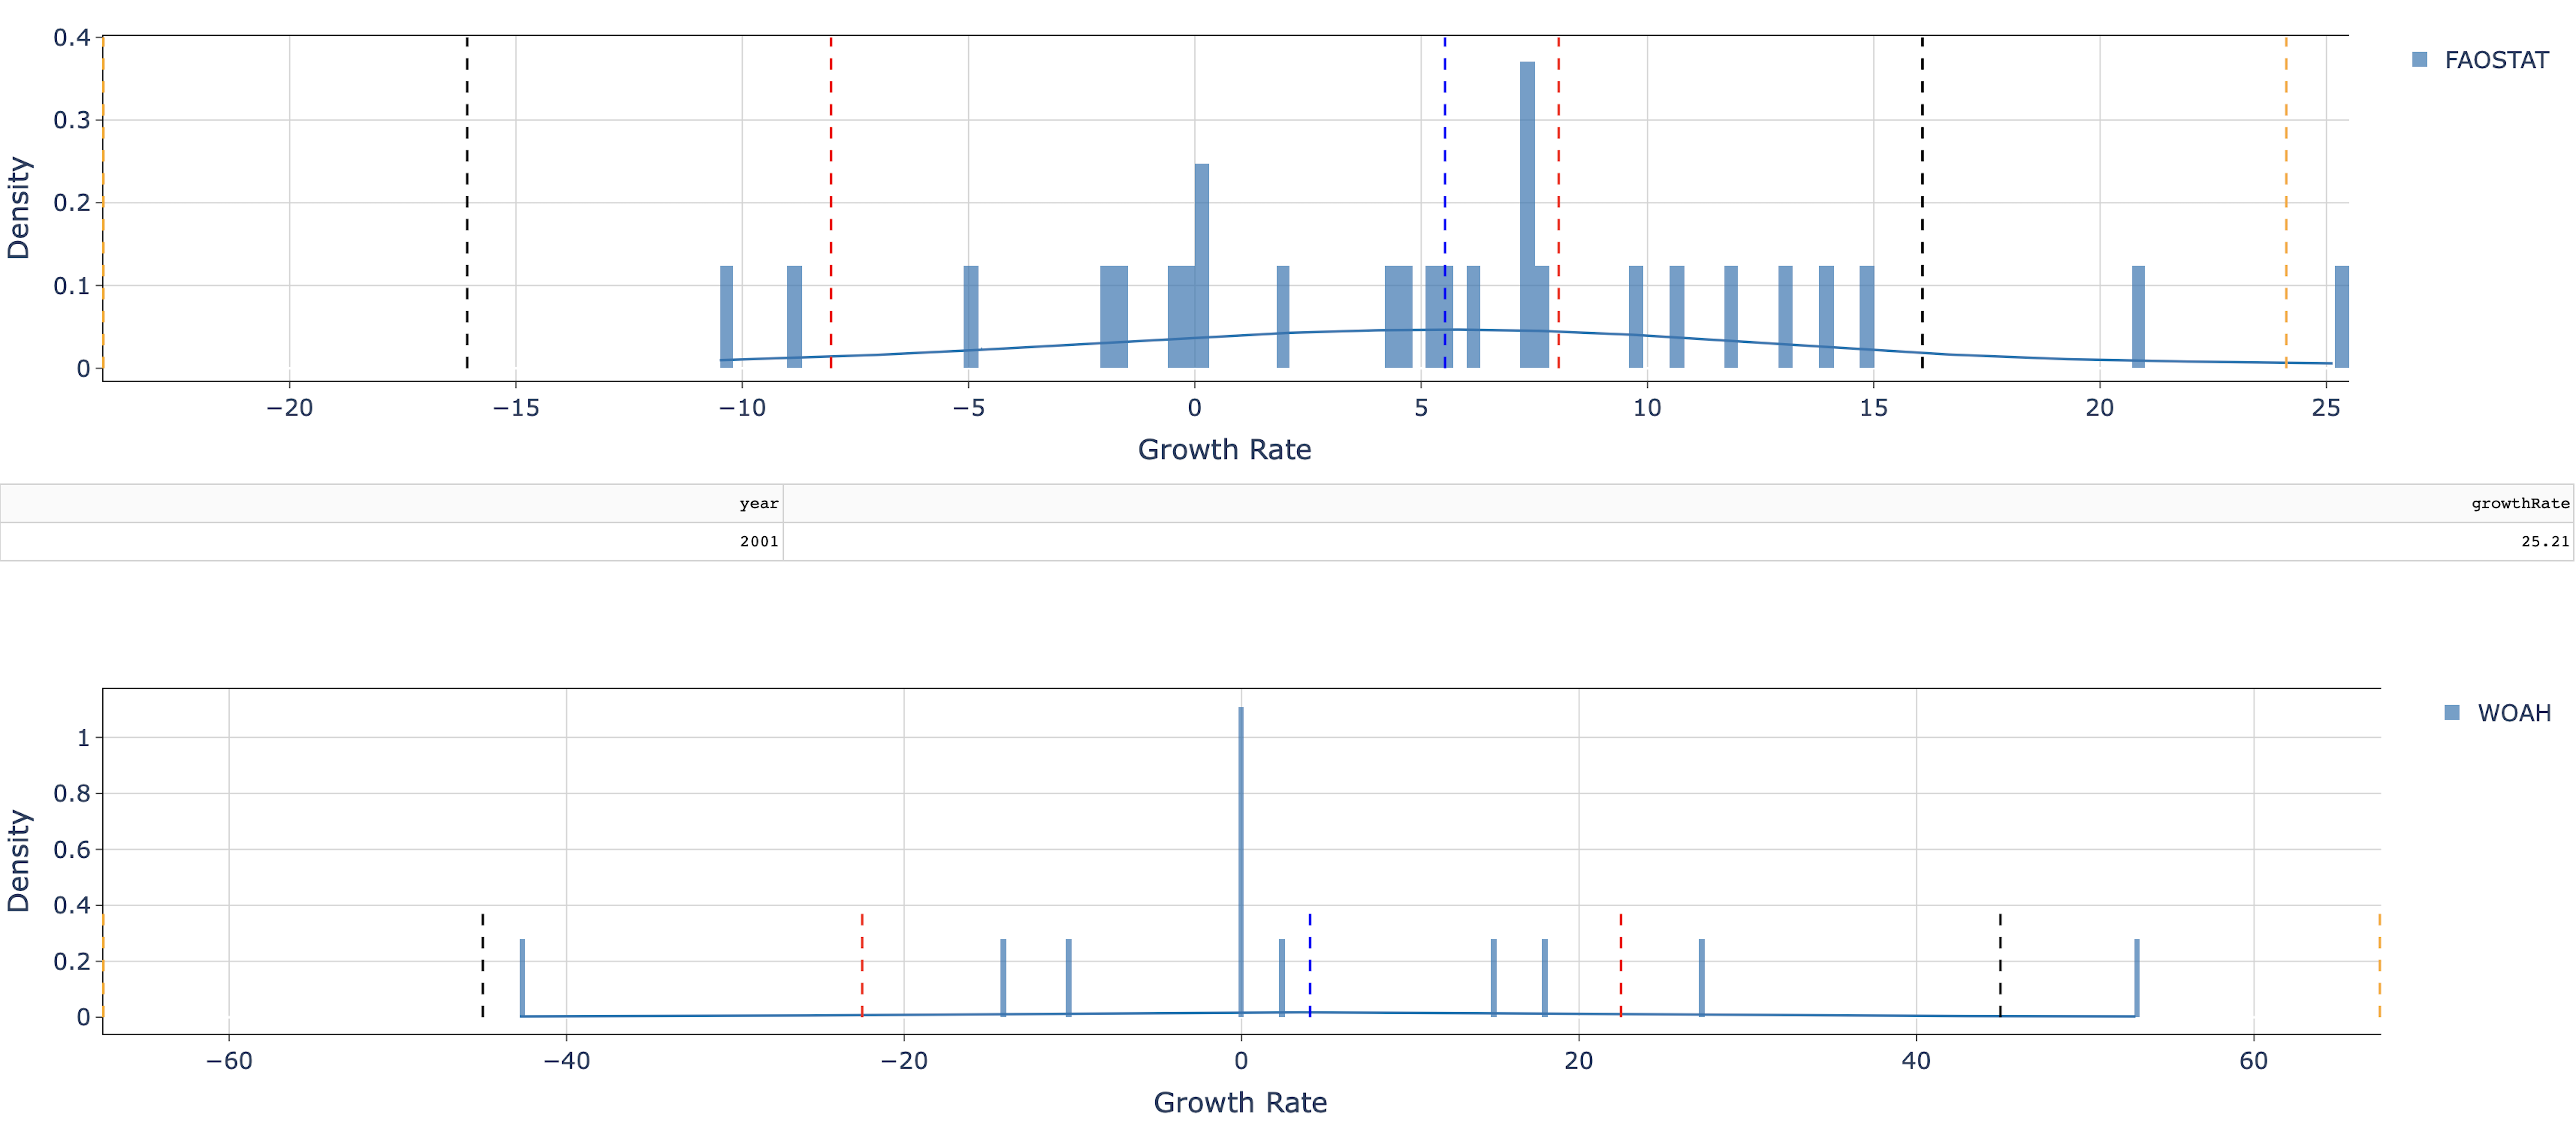
\includegraphics[width=1\textwidth]{image5}
    \caption{The growth rates for Sheep in Ethiopia from FAOSTAT (Top) and WOAH (Bottom) are plotted to normal curves. The first standard deviation line is red, the second standard deviation line is black, and the third standard deviation line is yellow.}
    \label{fig:image5}
\end{figure}

\subsubsection{Method 2: Interquartile range analysis}
The IQR is used to calculate the variance in magnitude for each quartile of the data. It also indicates outliers outside each data source's upper and lower fences. These fences visualize the first and fourth quartiles of data. These outliers can be easily seen and then investigated further. The IQR shows the median rate of change for the animal population, as well as shows the second and third quartile as boxes around the median. Figure~\ref{fig:image6} shows the spread of the yearly population rates of change for cattle in the United States of America. Assuming the population is large, good data should not have any outliers and the IQRs for each source should look similar to each other. 

%Image seven
\begin{figure}[h!]
    \centering
    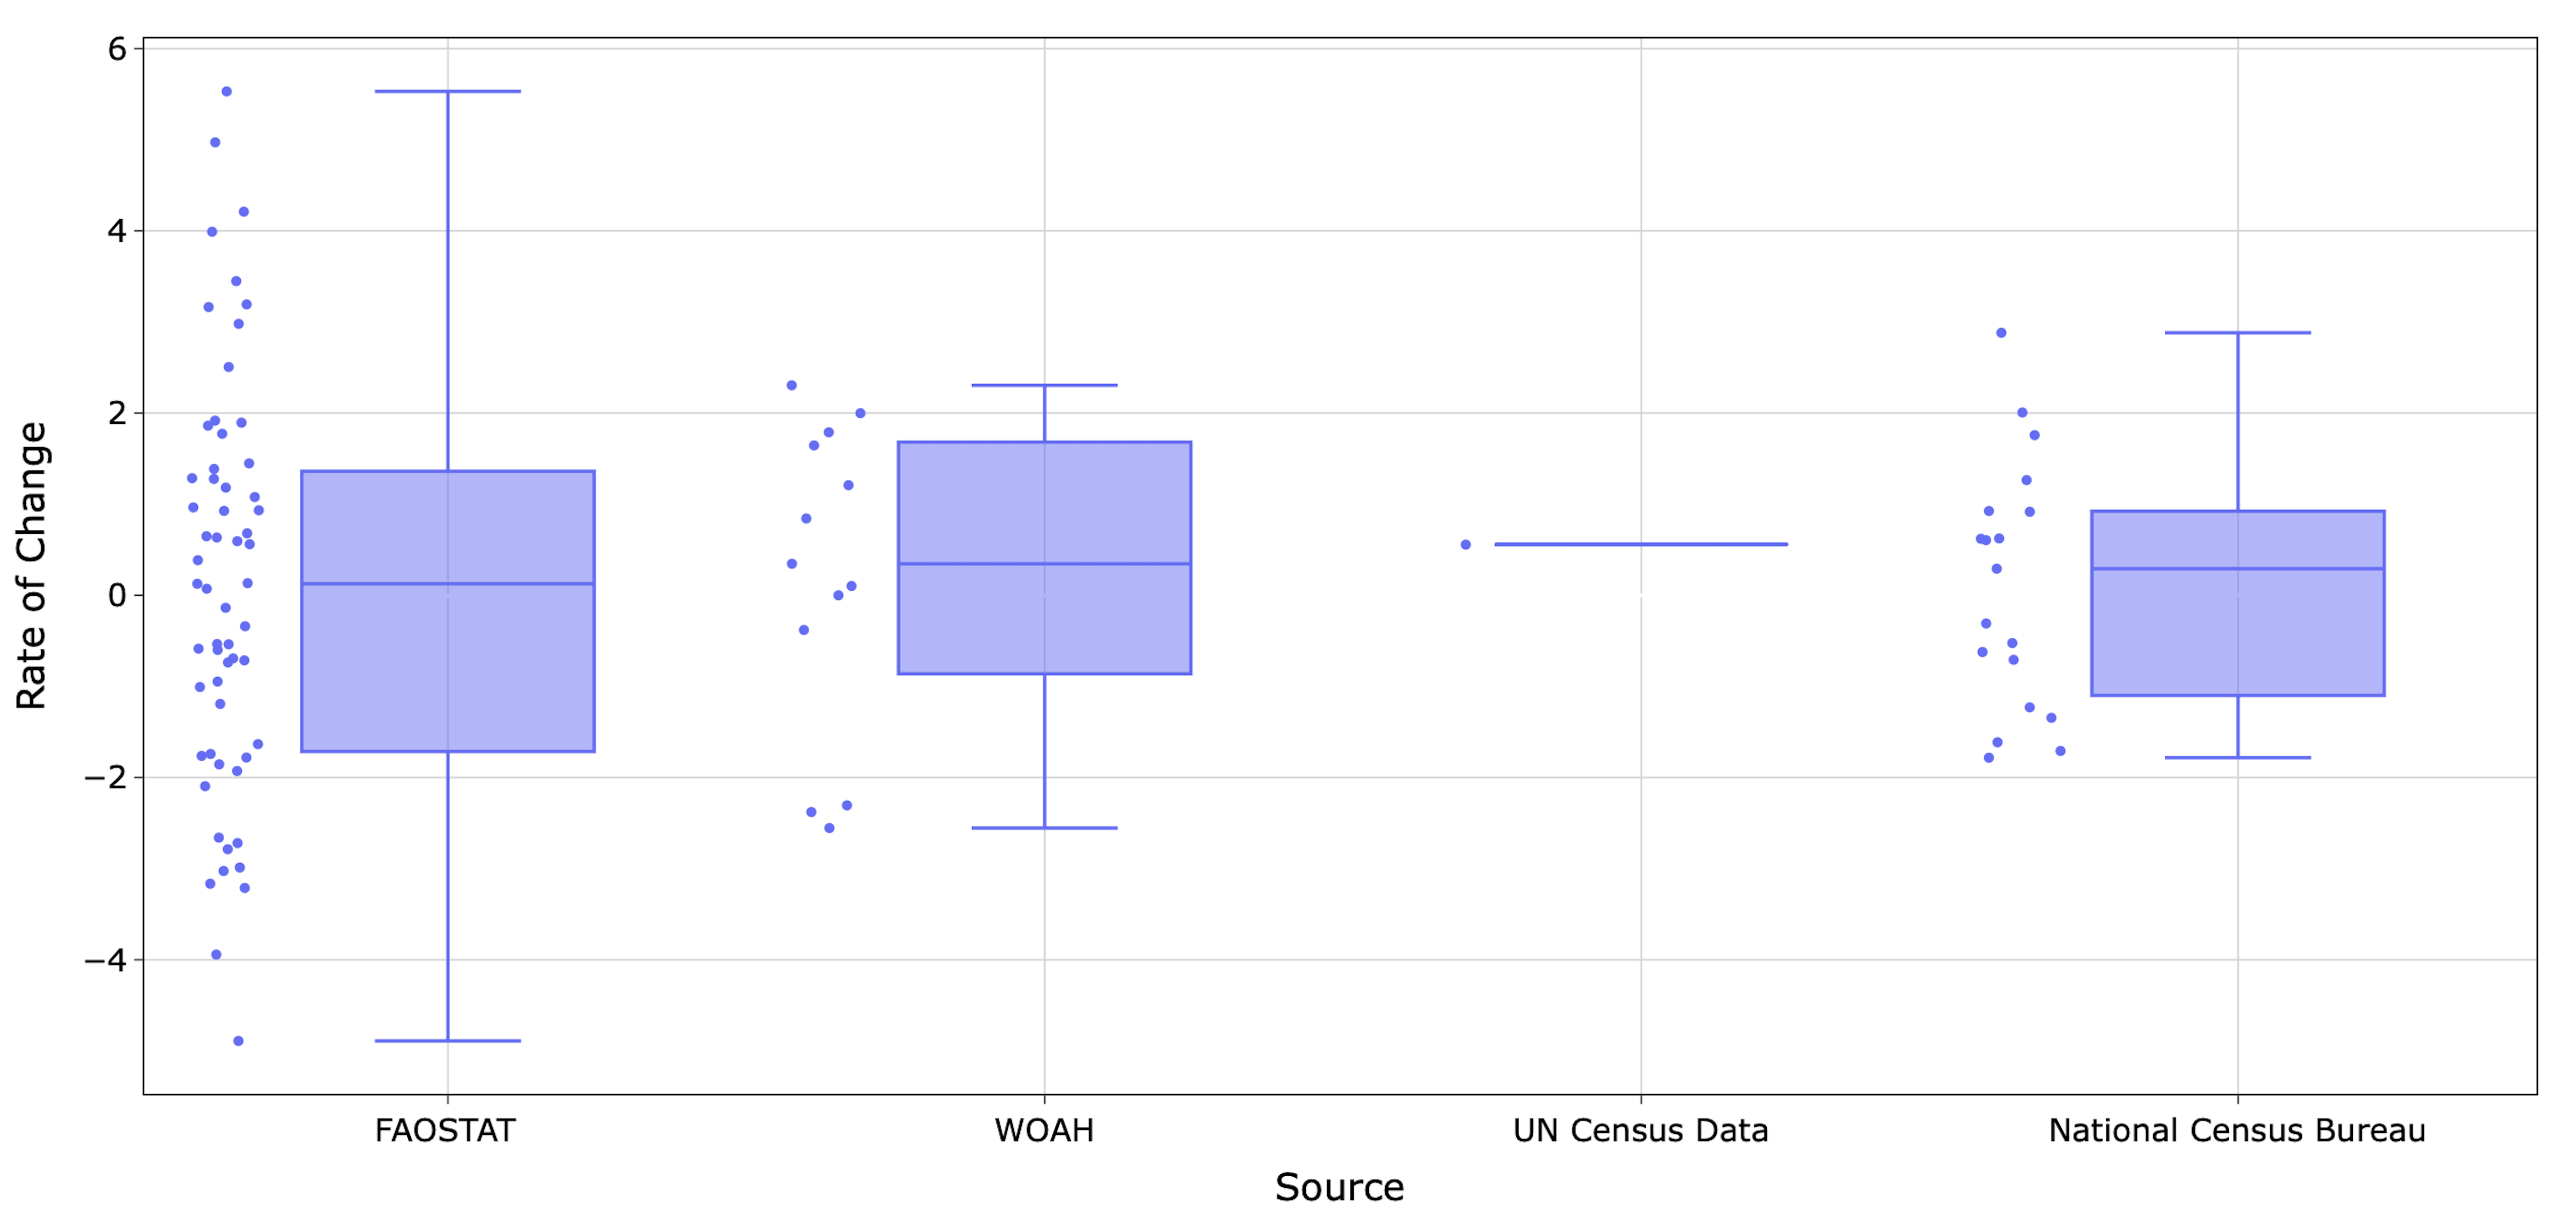
\includegraphics[width=1\textwidth]{image6}
    \caption{The interquartile ranges for cattle in the United States of America. Shows the interquartile ranges of the yearly rate of change in animal population numbers from the sources FAOSTAT, WOAH, UN Agriculture Census Data, and the National data from the United States. Note that the data from the UN Agriculture Census Data was taken in two different years, 2001 and 2012, so the rate of change was averaged across the 11 years. }
    \label{fig:image6}
\end{figure}

It is evident from Figure~\ref{fig:image6} that FAOSTAT has a much larger data spread for the rate of changes than the other sources. This could be because it has more data, so the uncertainty of the WOAH and national agricultural data is higher. Some examples of this are cattle in Greece where FAOSTAT data exists between 1960 and 2019 whereas WOAH data only exists between 2005 and 2015, or goats in Ireland where the FAOSTAT data also exists between 1960 and 2020 whereas WOAH data only exists between 205 and 2019. More evidence of this can be found using the general data viewer tool provided. Despite the differences in how much data is collected between all the sources, the median yearly rate of change is similar between all sources. 
The biggest difference between all three sources (excluding UN Agriculture Census Data due to its small sample size) is that FAOSTAT has much larger upper and lower fences. This is most likely due to FAOSTAT containing more data than either national agricultural data sources or WOAH. So, this indicates that there is a high probability that all three data sources are consistent and support each other. 

When comparing the rates of change for sheep in Ethiopia the IQR looks very different (see Figure~\ref{fig:image7}).
%Image eight
\begin{figure}[h!]
    \centering
    \includegraphics[width=1\textwidth]{image7}
    \caption{The interquartile ranges for Sheep in Ethiopia between 1960 and 2020. Shows the interquartile ranges of the yearly rate of change in animal population numbers from the sources FAOSTAT and WOAH.}
    \label{fig:image7}
\end{figure}
\begin{figure}[h!]
    \centering
    \includegraphics[width=1\textwidth]{image8}
    \caption{The interquartile range for goats in South Africa. Shows the interquartile ranges of the yearly rate of change in animal population numbers from the sources FAOSTAT and WOAH between 1960 and 2020.}
    \label{fig:image8}
\end{figure}

Figure~\ref{fig:image7} shows a large data spread for WOAH despite WOAH having less data than FAOSTAT. The second and third quartile of WOAH is almost twice the size of that for FAOSTAT. It also has long error bars and an outlier far beyond the top error bar. Excluding the outliers (assuming that they indicate an inconsistency), the data from WOAH for Ethiopian sheep is much less internally consistent than that of FAOSTAT. There are other examples of WOAH having data with extreme outliers. One example is goats in South Africa. In Figure~\ref{fig:image8} the extreme outliers are visibly showing a -90\% population rate for a single year with no other points coming close to it. Excluding the outliers (Figure~\ref{fig:image9}), it is clear that WOAH and FAOSTAT have similar median rates of change, but WOAH has only two years below the median. This is very surprising as it means it had almost half of the years surveyed at 0 percent population growth (this would not seem likely as animal populations usually change every year for a country of this size). FAOSTAT contradicts this as its median rate of change is 0.121 percent growth per year with no years of zero percent change. This illustrates a difference in the nature of the data recorded by WOAH and FAOSTAT.

%Image Nine and Ten
\begin{figure}[h!]
    \centering
    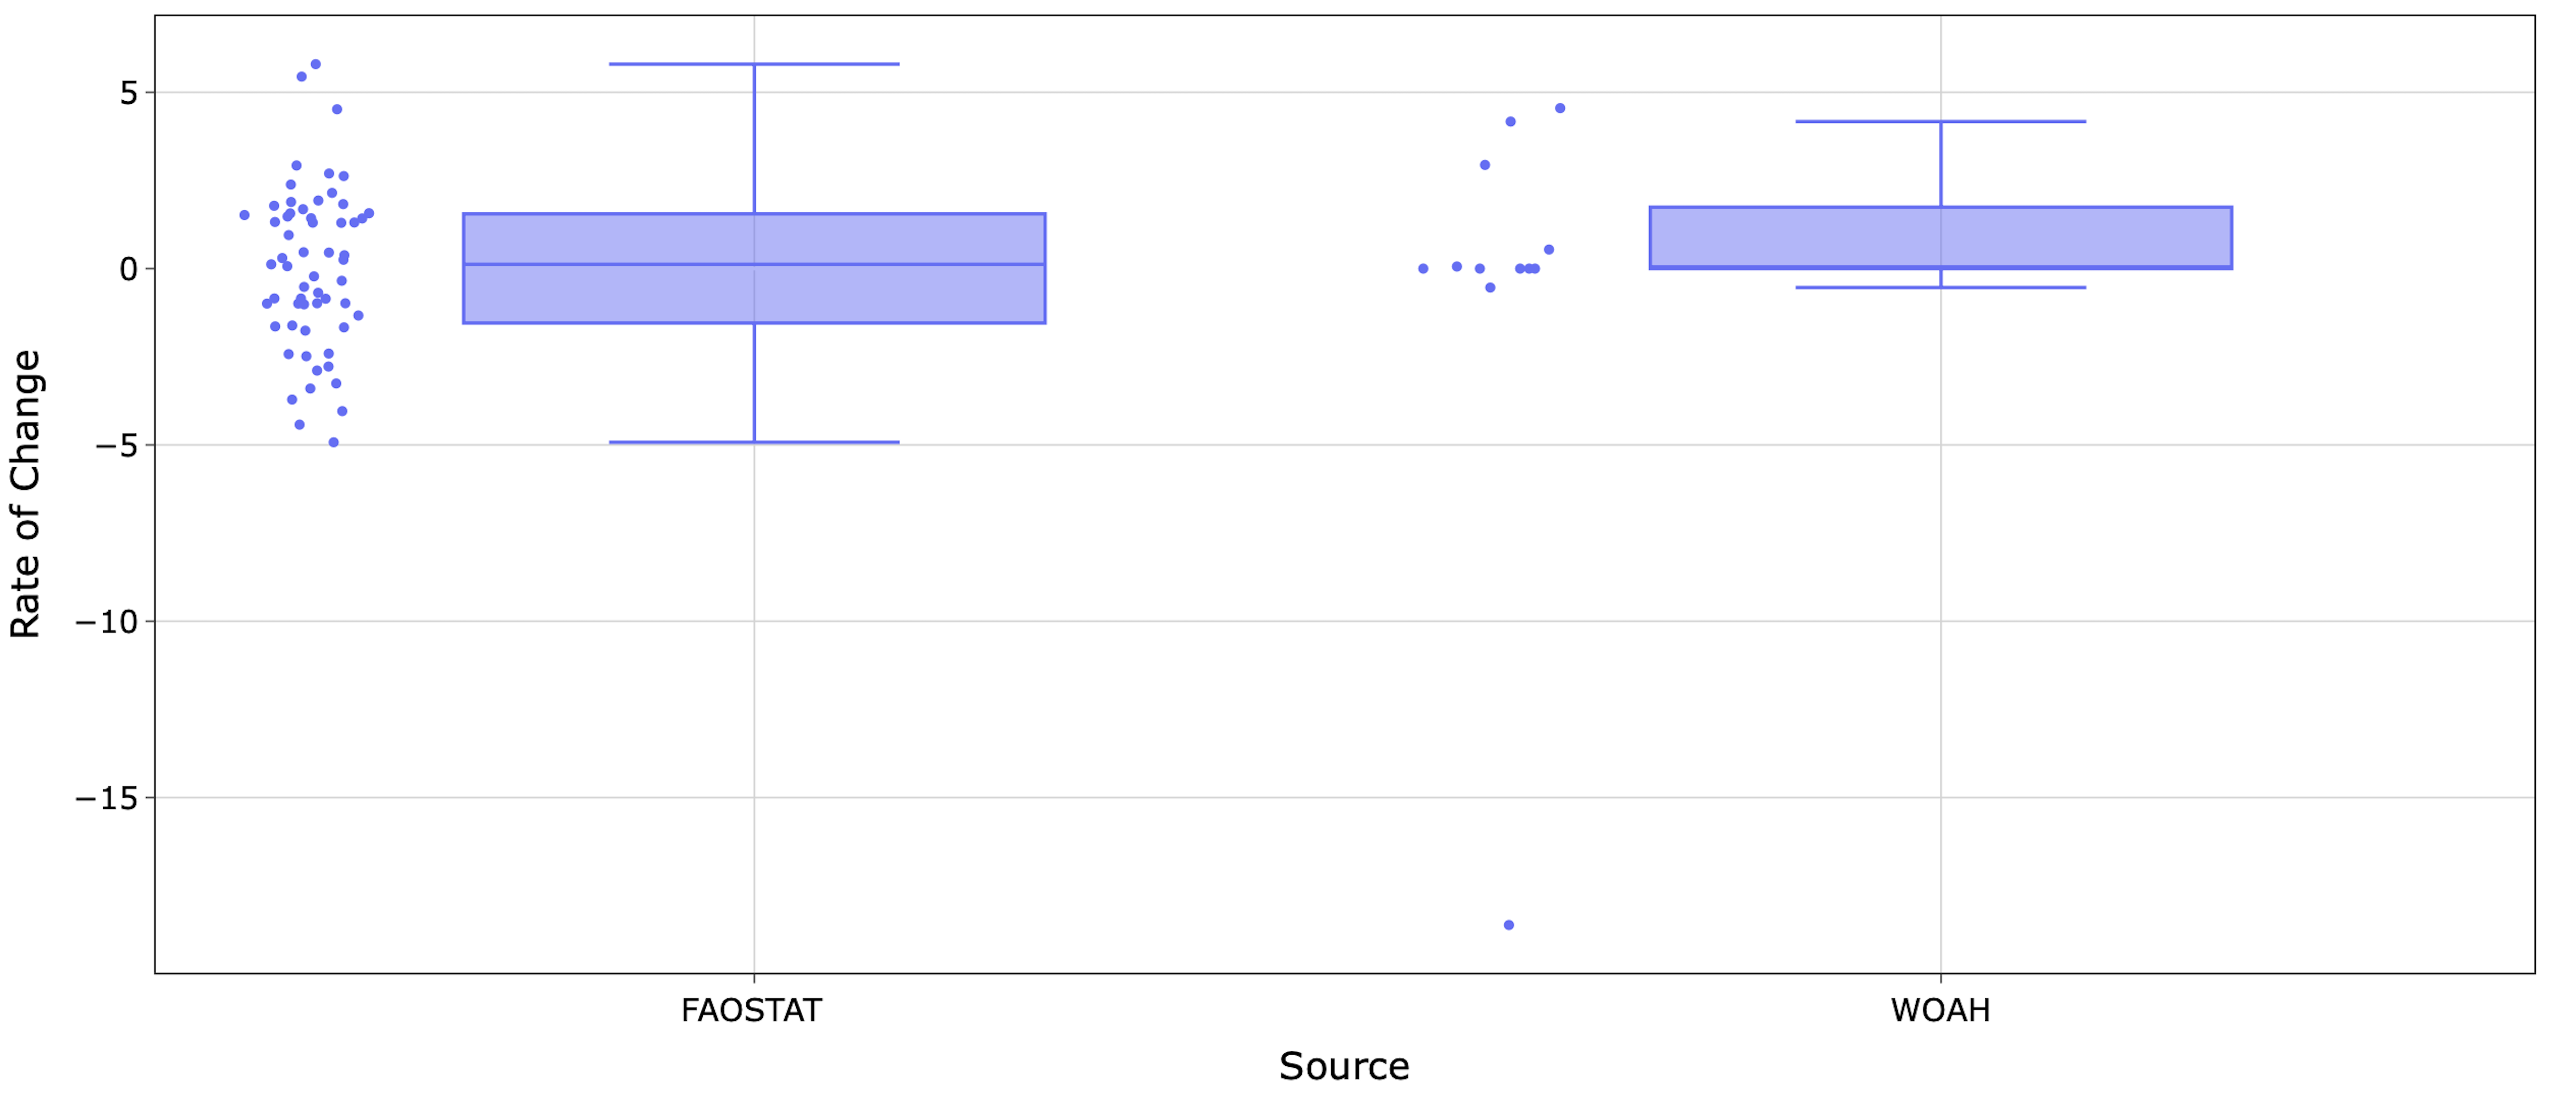
\includegraphics[width=1\textwidth]{image9}
    \caption{The interquartile ranges for goats in South Africa excluding the outliers.}
    \label{fig:image9}
\end{figure}

\begin{figure}[h!]
    \centering
    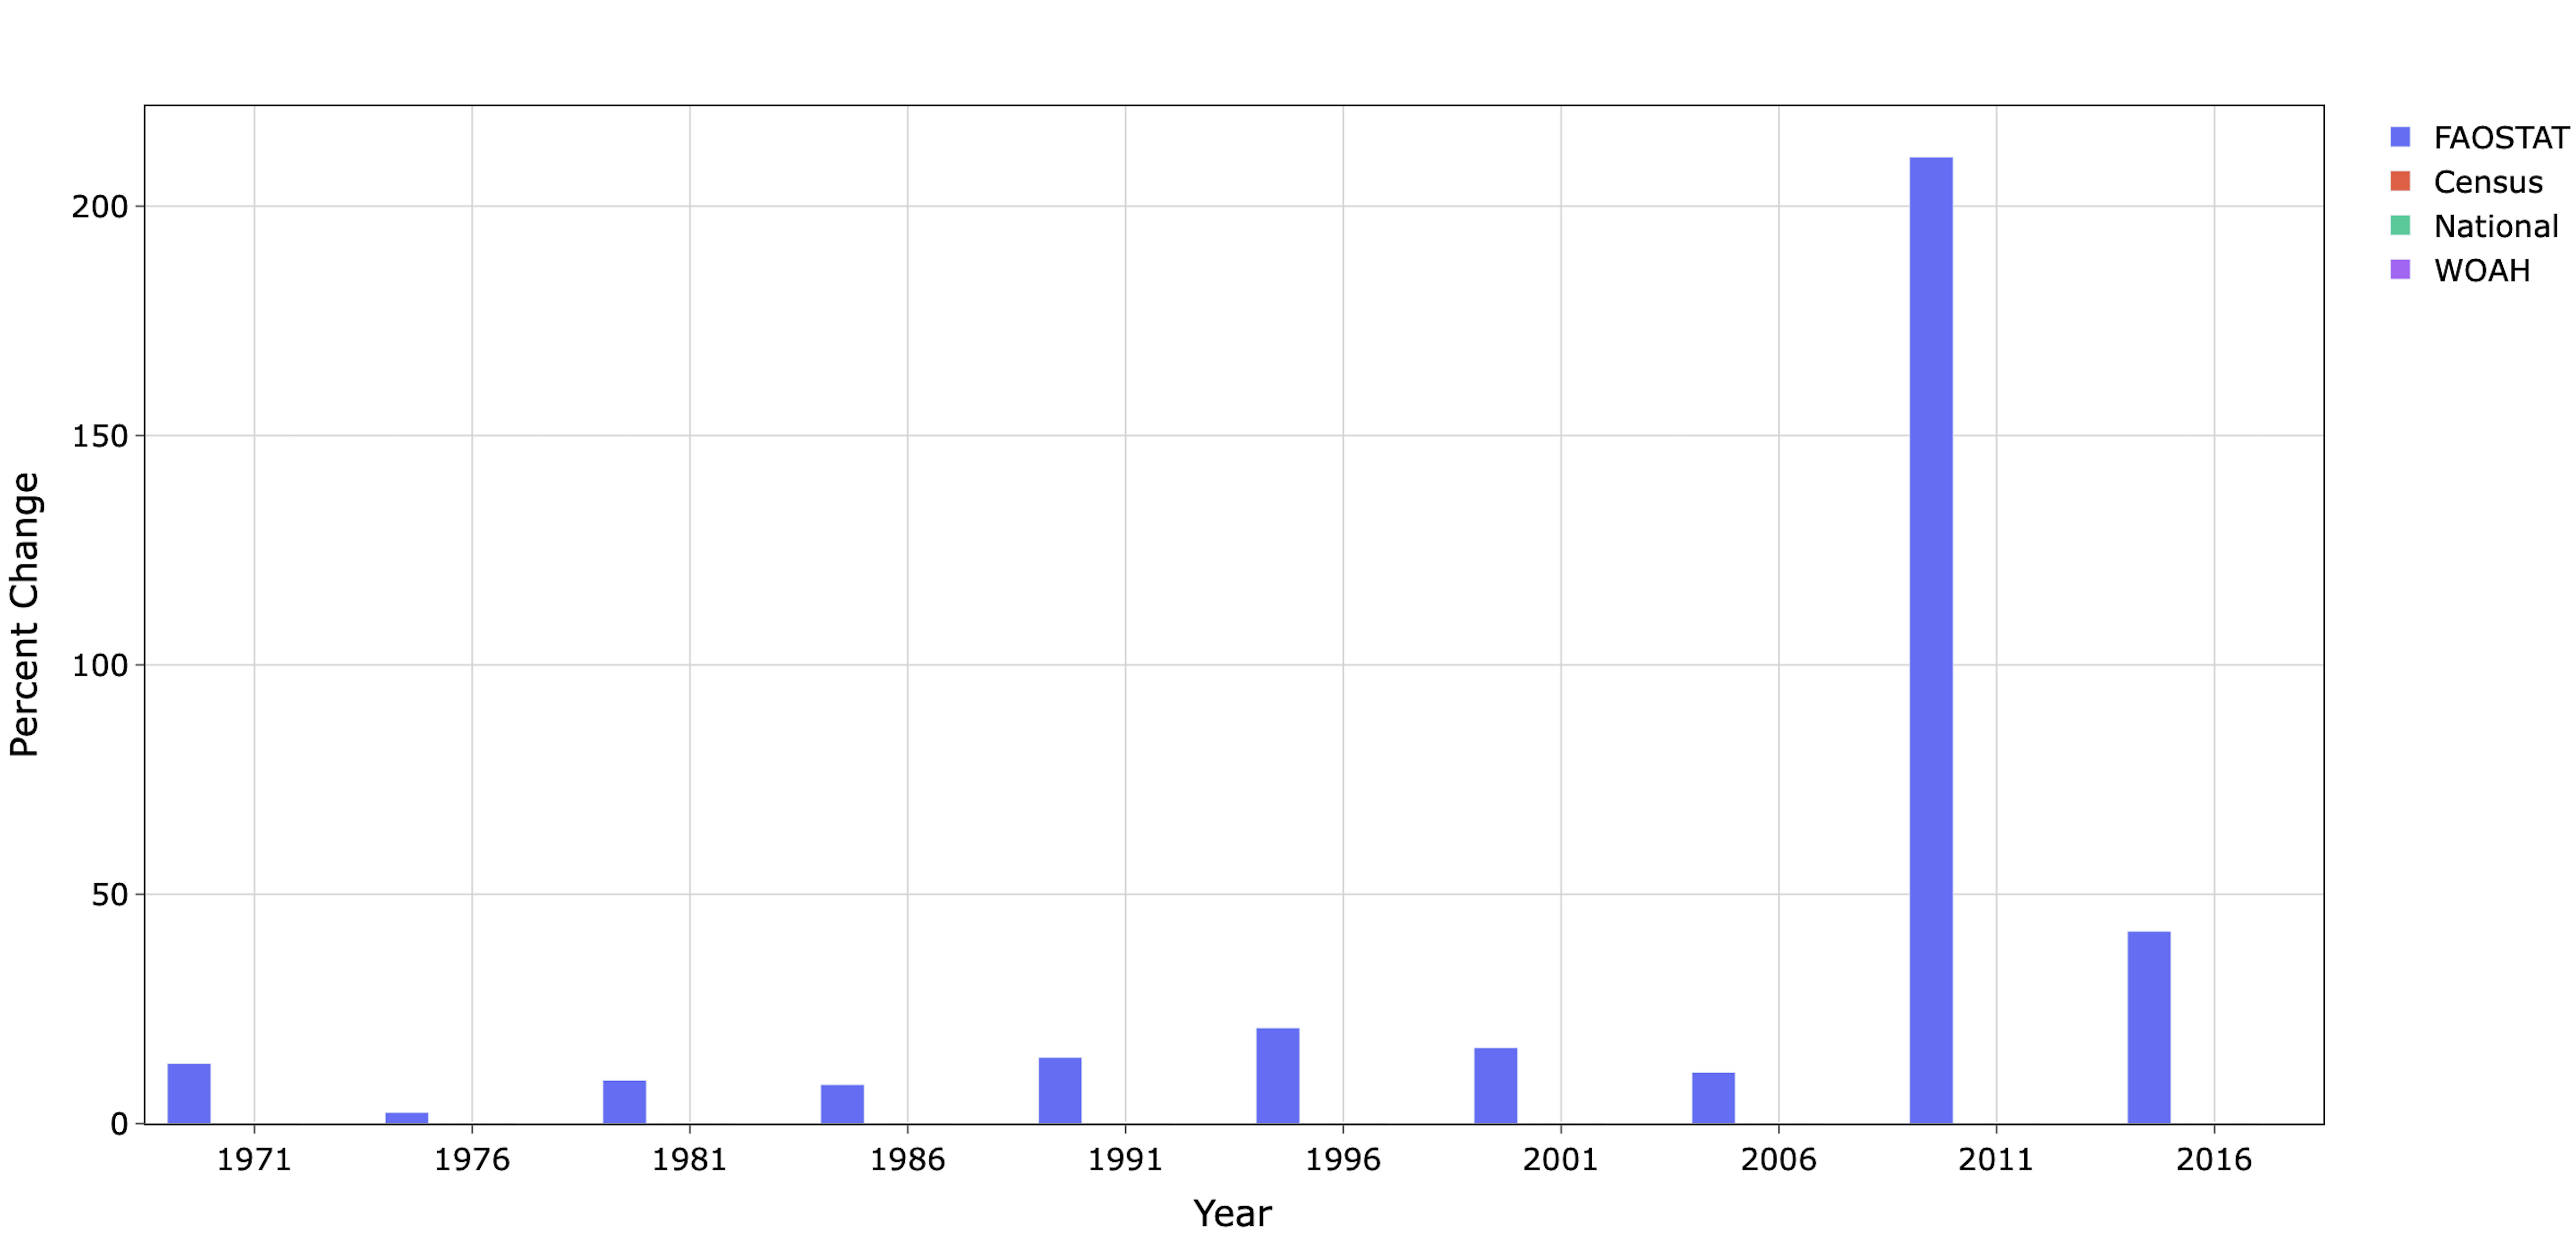
\includegraphics[width=1\textwidth]{image10}
    \caption{Finding the rate of change between two five-year averages for the chicken population in the United States of America.}
    \label{fig:image10} 
\end{figure}

Figure~\ref{fig:image9} shows the interquartile ranges for goats in South Africa and there are some clear outliers in the data for WOAH. Figure~\ref{fig:image10} shows the same data excluding the outliers and shows a fairly similar IQR box plot showing the data is mostly identical. The only other possible inconsistency is that WOAH has 4 data points with zero rate of change. Investigating the WOAH data points further exposes some suspicious data points. 2005-2007 has the exact same population between all years and 2008-2010 also has the exact same population between the years. However, 2018 is most likely the largest data inconsistency because that year WOAH reported 54.2 million goats in South Africa which is suspicious since it reported 5.4 million goats. Since FAOSTAT reported 5.4 million goats that year it is almost certain the WOAH put the decimal place in the wrong spot and actually meant to report 5.42 million goats. 

\subsubsection{Method 3: Trailing five-year analysis}

The final analysis performed on the data sources was by finding the trailing five-year population averages across all four data sources. Then the rate of change between a trailing five-year average and the previous trailing five-year average is found. This process is performed for each data source on all trailing five-year groups of data and then plotted to identify the differences. This method of analysis was chosen for our study because it will show the average growth over five years. This will show general trends more than sudden yearly changes. If for one year there was a large growth of an animal population and the next year that animal population declined by the same amount, over the trailing five-year span the average will not reflect these sudden changes. So, if this does show a large change over those five years then it is evidence that that time span should be investigated further as there would have been something influencing that period to have such change.
An example of the usefulness of this analysis is seen in an examination of the chicken population in the United States of America.
It is clear from Figure~\ref{fig:image10} that there was more than 200 percent growth between the trailing five-year averages ending in 2006 and 2011 for FAOSTAT. This is far beyond what is normal for this time range when comparing the years' rate of change to the historic rates of change. The half-decade following also had nearly 50 percent growth showing this population growth was not a one-off incident. It can be determined from this either the United States of America massively increased its chicken population post-2006, the method for counting chickens was changed during this time, or there is an inconsistency in the data.

%Image 11
\begin{figure}[h!]
    \centering
    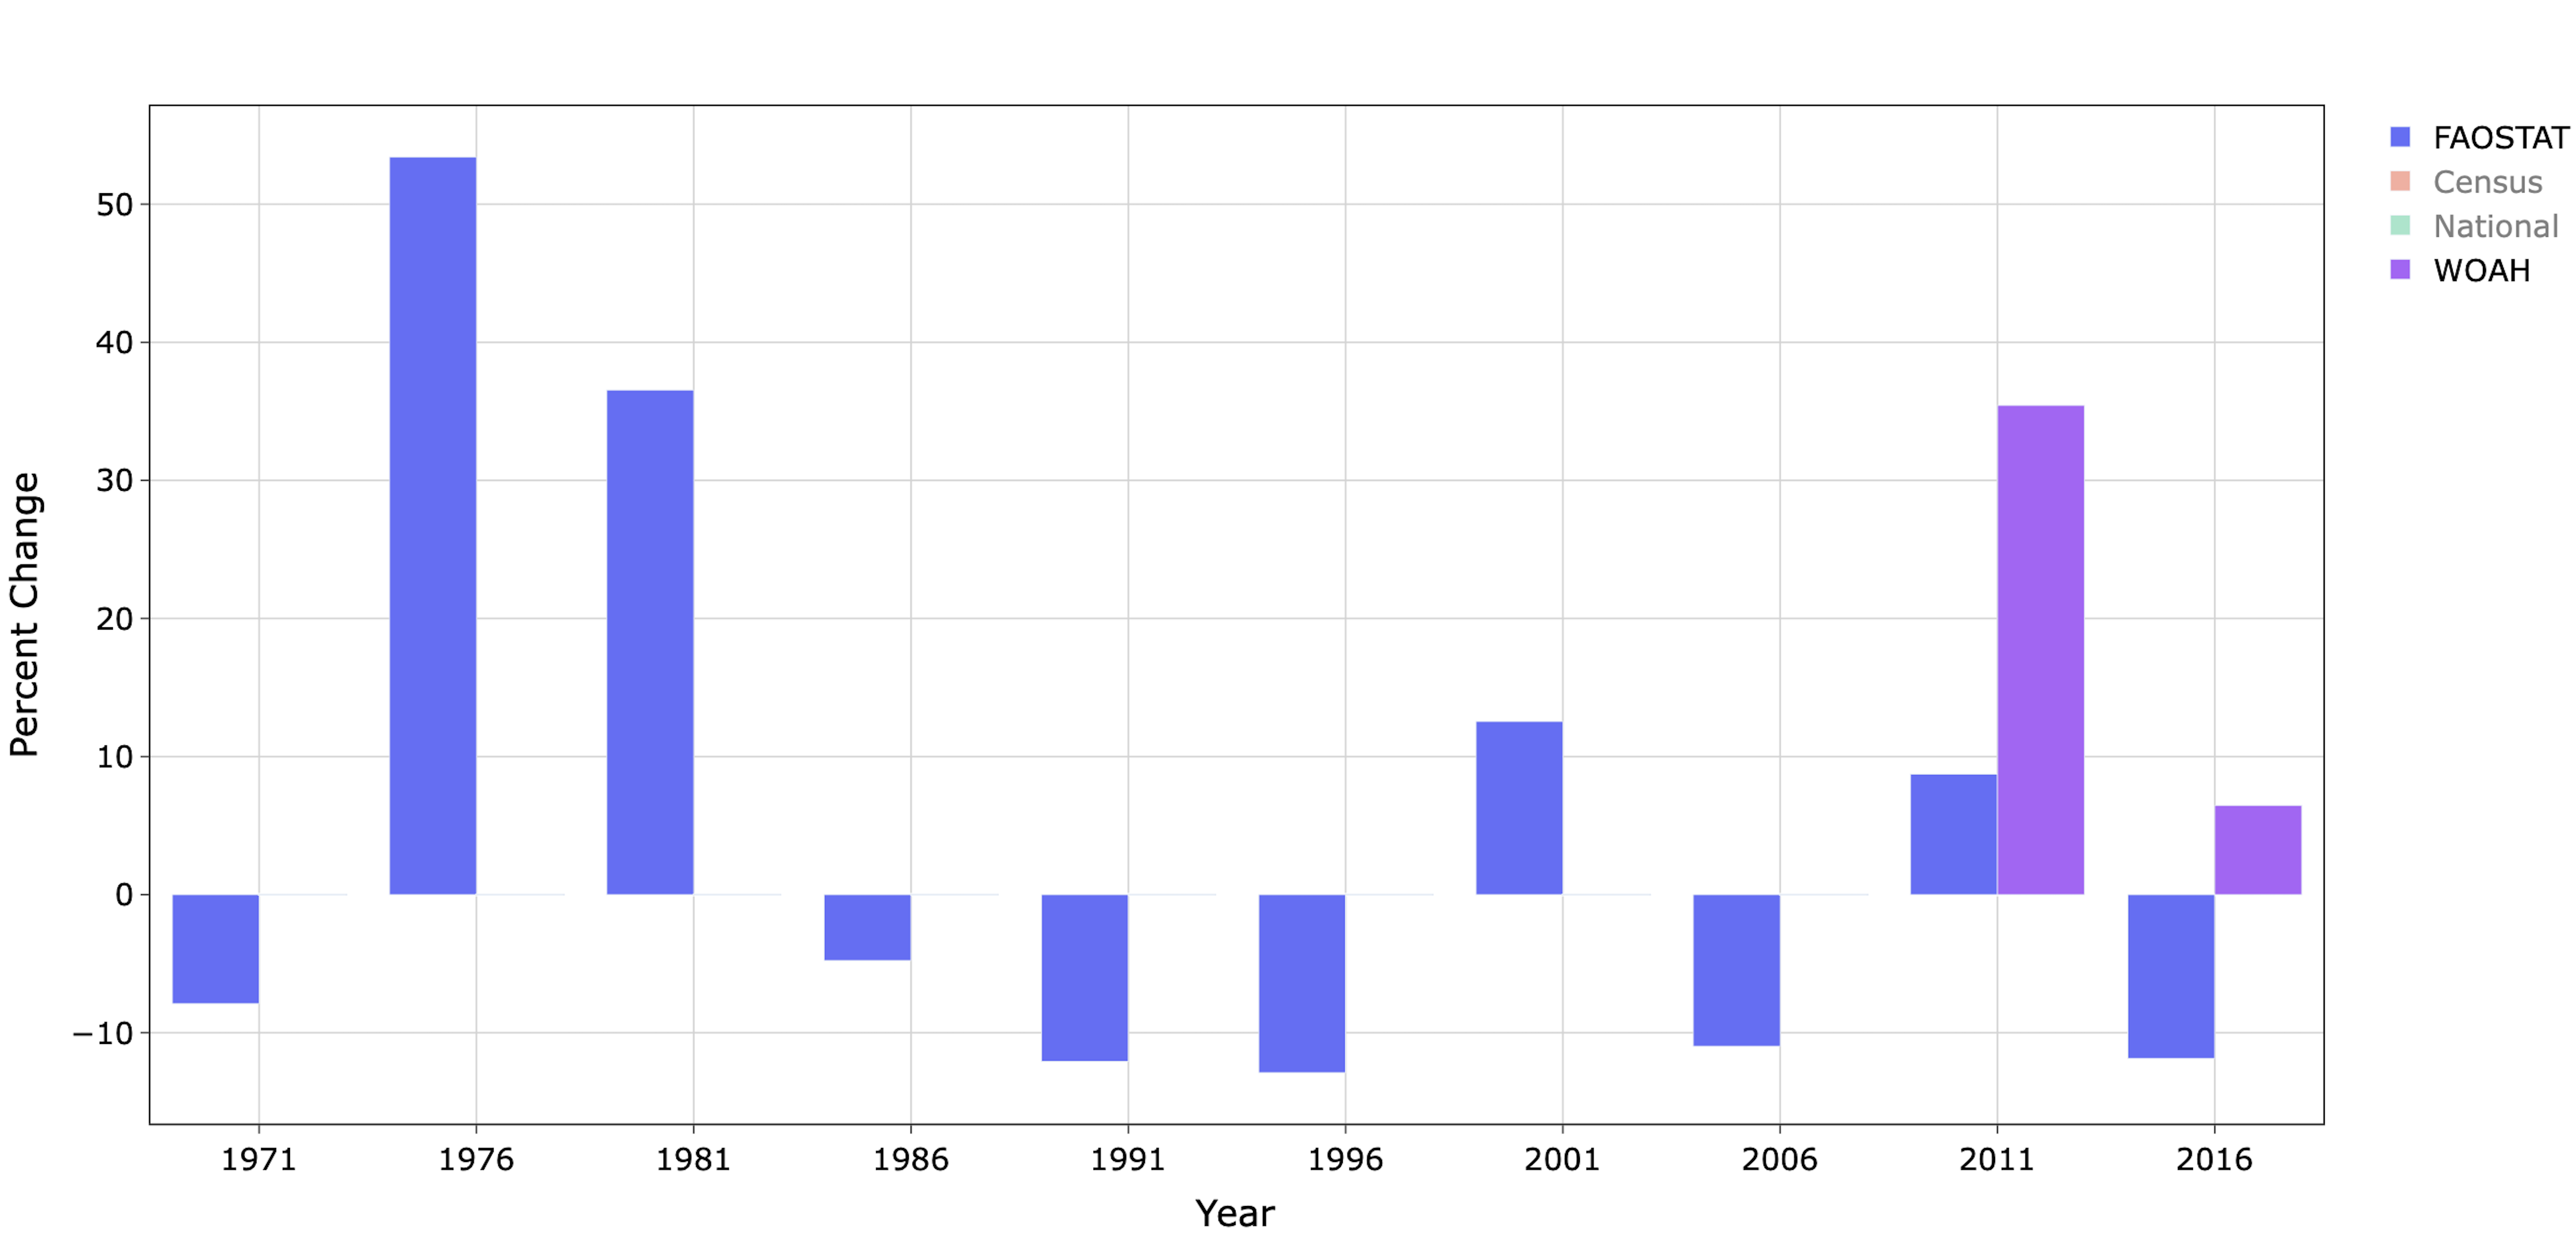
\includegraphics[width=1\textwidth]{image11}
    \caption{The rate of change between trailing five-year averages for the cattle population in Botswana for the sources FAOSTAT and WOAH}
    \label{fig:image11}
\end{figure}

%Image 12
\begin{figure}[h!]
    \centering
    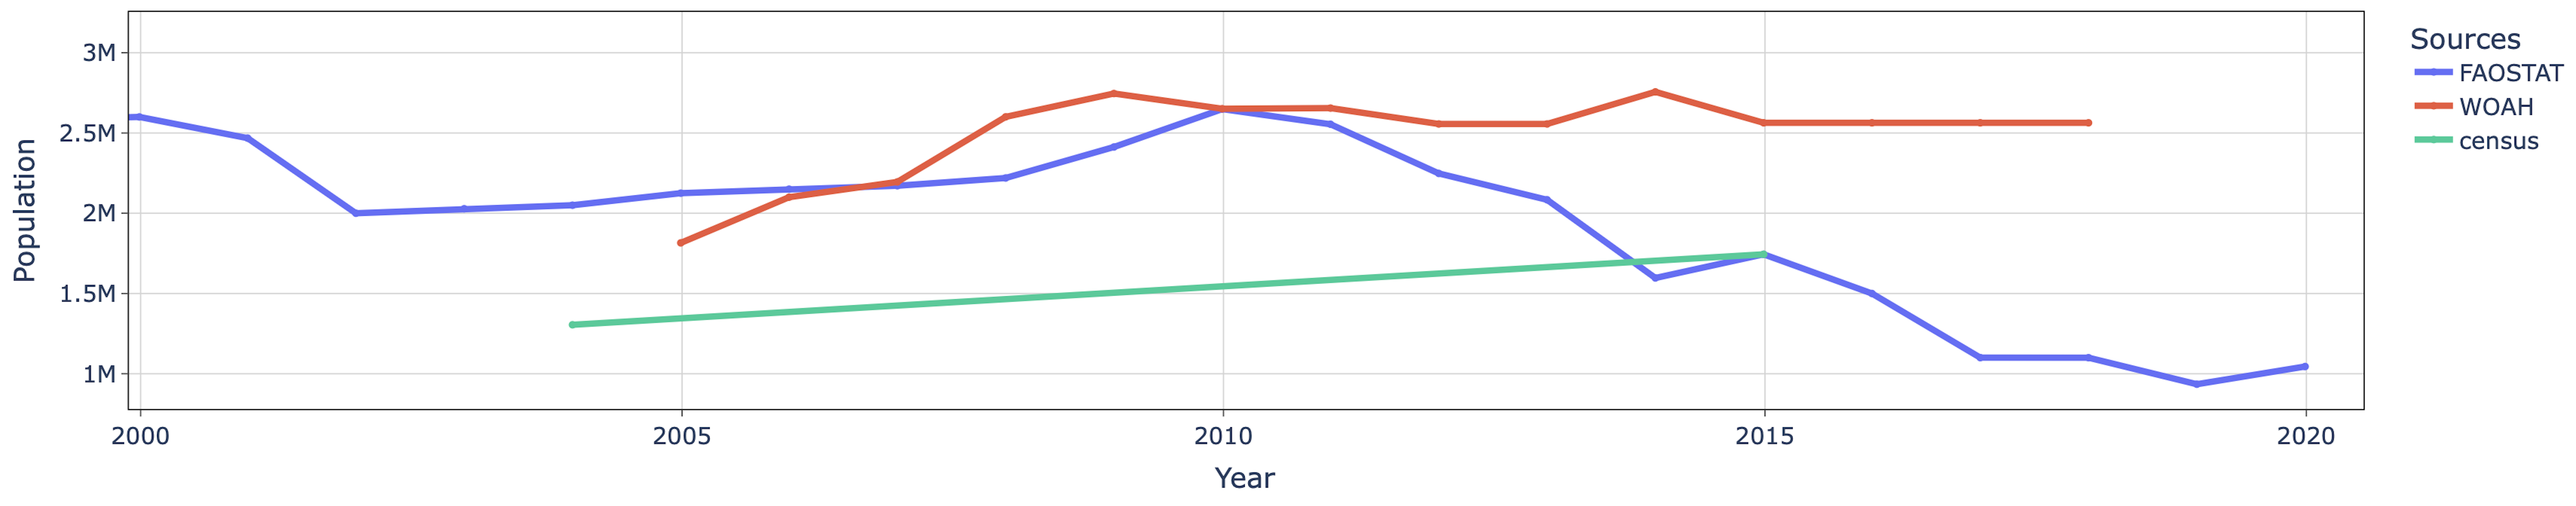
\includegraphics[width=1\textwidth]{image12}
    \caption{Shows the population of cattle in Botswana between 2000 and 2020 for FAOSTAT, WOAH, and UN Agriculture Census data}
    \label{fig:image12}
\end{figure}

Figure~\ref{fig:image11} shows the cattle population in Botswana. In the FAOSTAT data, it is clear that the population has periods of rapid growth then stagnation and decreasing population numbers. However, the data from WOAH shows a brief data period where the population has been growing at a much faster rate than what FAOSTAT has shown over the same period. WOAH shows the population growing very fast between the 2006 and 2011 averages, with almost 35 percent growth over the half-decade. This is in stark contrast to FAOSTAT which shows an 8 percent decrease in population over that same period. That’s a large difference! Consulting the actual animal populations in Figure~\ref{fig:image12}, it is clear that the animal population measurements between both sources are rarely identical and WOAH's numbers are stagnant between 2012 and 2018. This is the opposite of what FAOSTAT is reporting with a large decrease in cattle populations over that same period. Between these two data sources, it is very hard to tell which source is most accurate. WOAH may be more accurate as it shows a population more similar to the pre-2005 population average for FAOSTAT. But, FAOSTAT and the UN Agriculture Census data are identical in 2015 which indicates that these population numbers have support as well. This shows that it is difficult to determine what is the most 'reasonable/representative' population numbers for cattle in Botswana. 


\begin{figure}[h!]
    \centering
    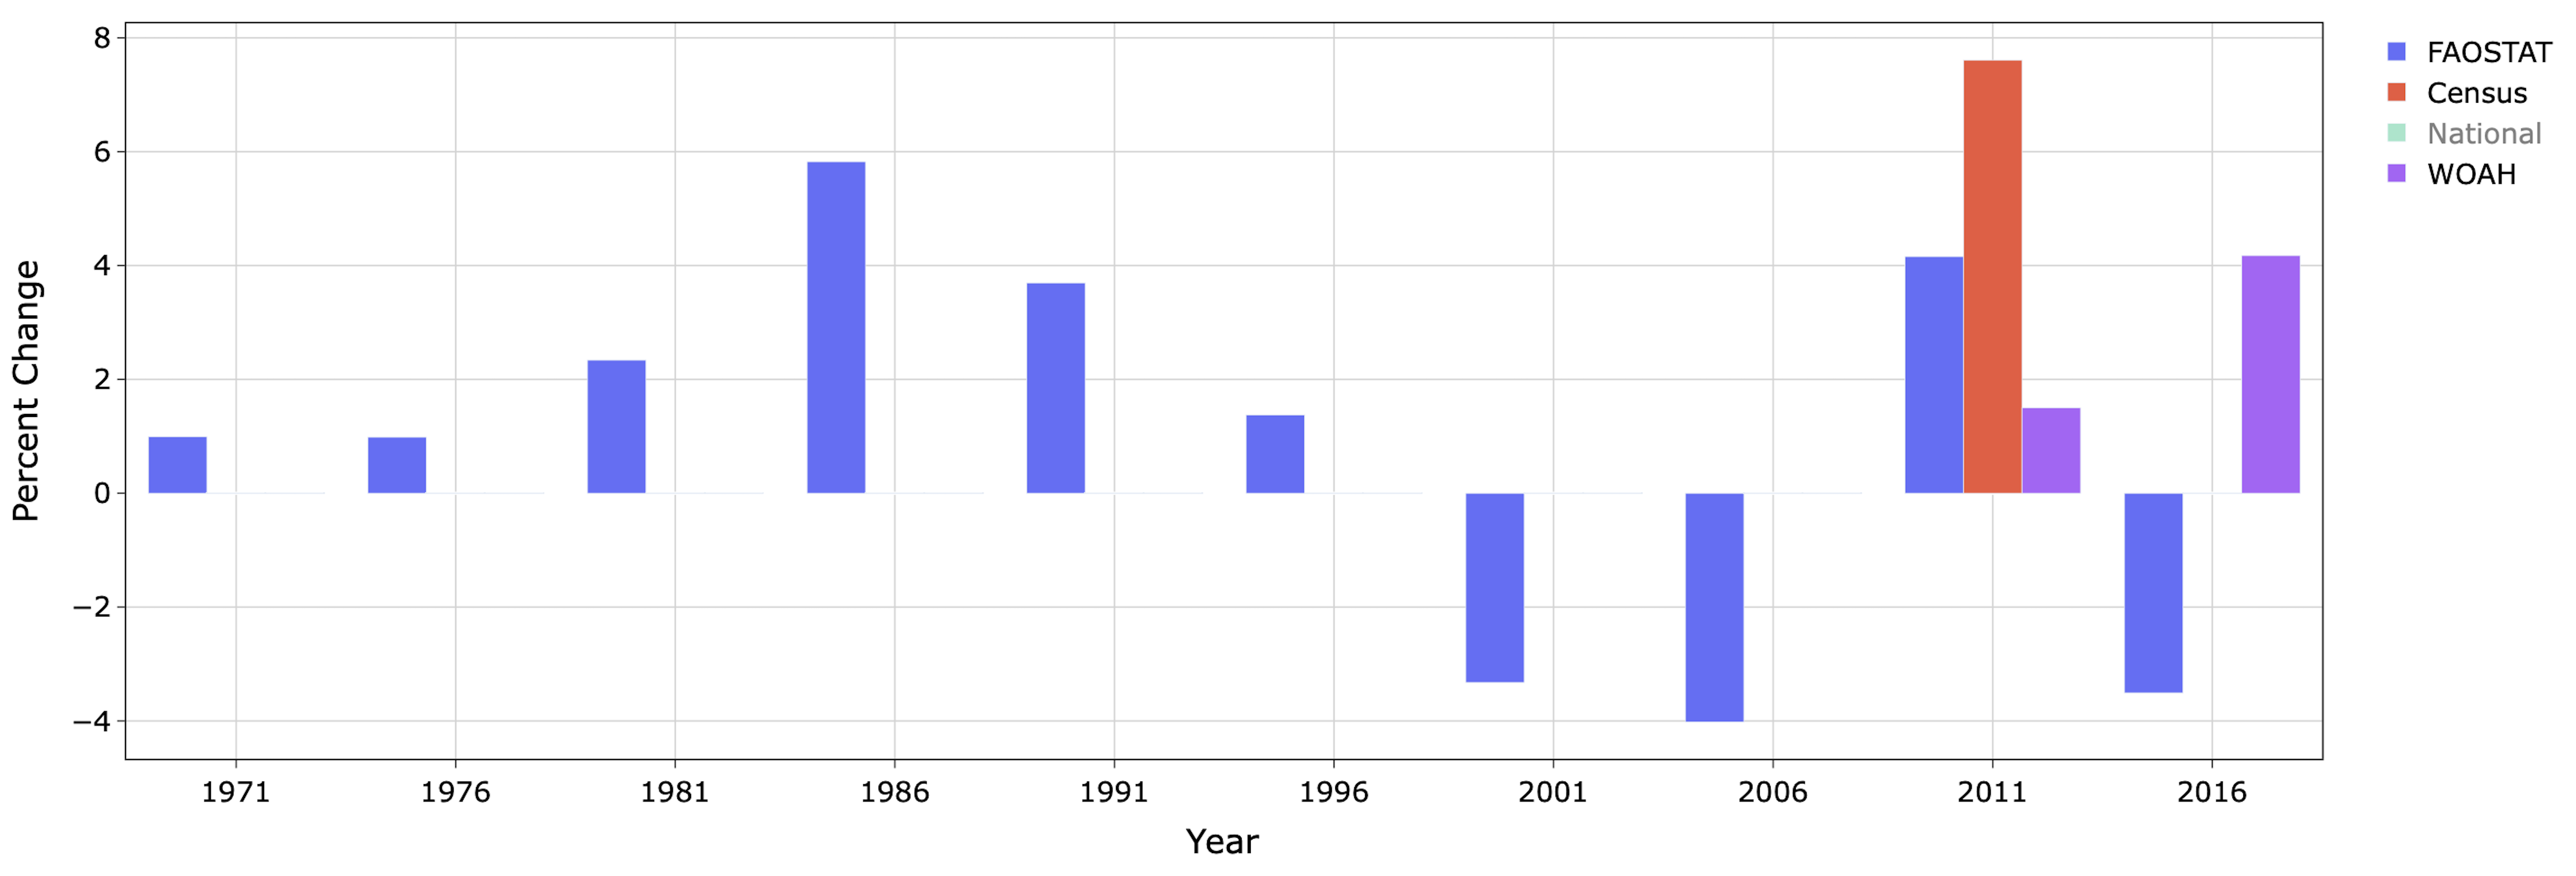
\includegraphics[width=1\textwidth]{image14}
    \caption{Finding the rate of change between two trailing five-year averages for the cattle population in India}
    \label{fig:image14}
\end{figure}

Figure~\ref{fig:image14} shows the cattle population in India (excluding buffaloes and mithuns) and it is clear that the three sources have very similar data. Each change for a trailing five-year average is less than 10 percent between its peers so this is a very reasonable rate of change. FAOSTAT data also follows a reasonable curve having few massive gains and drops between years. This is a good example of what consistent data should look like. This shows that FAOSTAT, WOAH, and UN Agriculture Census data can be similar and corroborate animal population numbers for specific years and specific countries. 

\subsection{Possible reasons for inconsistencies and their effect on the data}

There are many different reasons animal population numbers can fluctuate and not follow a linear path. Such examples can include policy change, environmental circumstances, diseases, untruthful responses from surveys, and more. This section will investigate some documented reasons that can explain why some inconsistencies are truthful. This is important to document because it shows that the data points outlined in the table in section 7.1 may not be wrong or inconsistent, but rather need investigation to explain why the data is behaving in unexpected ways.

The ability to automatically identify potential inconsistencies allows users of the data the ability to investigate and determine whether there is a reason for the peculiarities that may arise in the data.

There are other possible reasons for inconsistencies that are not unique to livestock population data. There can also be issues in distribution that can affect the data being presented to users. A decimal point could be entered in the wrong location, or updated data could be entered in the wrong spot. Data could also be mislabeled. These are possible mistakes of many that can happen regardless of what data is being provided.

\subsubsection{Policy change}
With the growing need for countries to reduce their environmental footprint and the high level of greenhouse gas emissions from livestock production, many countries are incentivizing farmers to reduce their livestock population \citep{lyman_incentivizing_2013}. For instance, when Czechoslovakia split into Czechia and Slovakia in 1993 and each country joined the European Union (EU) in 2004. In the 2000s, the livestock populations of Czechia and Slovakia declined. At face-value, the decline may appear to be a hangover from the split between the two countries (\textit{e.g.} hurt livestock sectors, issues reporting livestock in new government structures, changes in data infrastructure and reporting). However, upon joining the EU, countries are required to be compliant with the EU's environmental regulations (\textit{e.g.} reducing livestock populations, re-wild land, switching to growing crops with lower environmental impact), leading to changes in livestock structure and populations. By identifying the inconsistencies in the data, the decline in livestock population in Czechia and Slovakia post-split could be investigated, showing that countries attempting to be compliant with the EU's sustainability goals can impact the trend of livestock population over time. 

\subsubsection{Inaccurate livestock population surveys}

Data collection methods, such as paper surveys, may impact the reliability and accuracy of data. For example, surveys performed by governments often require farmers to fill out a form to report data about their herds. However, farmers may underestimate the livestock population in fear that the government may tax them more, leading to inaccurate or underestimated livestock populations for a country. This has been reported in Australia, where there is evidence that in the national livestock census, their cattle population is underestimated\citep{geoffry_fordyce_australian_nodate}.

Cultural differences in the significance of the value of livestock may also contribute to inaccuracies in livestock population surveys. For example, pastoralist communities in Ethiopia sometimes do not have access to bank accounts and instead, keep their wealth in the animal herds that provide their income and livelihood \citep{catley_livestock_2014}. 
So when asking these groups the population size of their livestock, it is like asking somebody what is the balance of their bank account which is very private, so they could give false answers to keep it private or make themselves appear more wealthy than they actually are \citep{catley_livestock_2014}. Some cultures also believe talking about herd size can bring bad luck \citep{international_wool_textile_organization_sheep_nodate}. All these factors can make herd owners hide the true sizes of their herds.

Some sources also do some minor editing on the data to make the data more reasonable. FAOSTAT will add missing dates and perform some corrections on incorrect data to make a complete dataset \citep{faostat_2019}. This is to fill in data between missing dates from a country or for errors such as an incorrect decimal point. They then add flags on the data to indicate if a data point is official, unofficial, forecasted, or imputed. WOAH in contrast does not change the data they receive from countries since they view themselves as a data distributor, not collectors or editors.

\subsubsection{Environmental factors}
Drought can affect population numbers due to the mortality of animals and because farmers can submit false numbers to get greater government assistance. Some countries are especially prone to drought as they lie in arid areas where rain is the primary source of fresh surface water. One example of this is Ethiopia where malnutrition or dehydration and other effects of drought caused between 61 and 100 percent of excess livestock deaths during drought periods \citep{catley_livestock_2014}. This can cause sudden drops in livestock population counts and this can be seen in livestock surveys. Governments may seek to replace livestock lost during natural disasters to support their farmers. As a result, some farmers report higher mortality than what actually occurred to receive more support and resources from their government \citep{catley_livestock_2014}. These can all cause sudden changes in livestock population numbers that might appear inaccurate when compared to past and future population numbers but are true.

\subsubsection{Diseases}
Livestock infected with disease can impact population trends due to large-scale culling events to eradicate or prevent disease spread. For example, the 1985 Bovine Spongiform Encephalopathy (BSE, also known as "mad cow disease") outbreak in the United Kingdom led to high levels of cattle infected by BSE. The outbreak resulted in beef and cow import bans from the United States and the EU due to the hazards to other livestock and human safety. As a result, Britain culled and incinerated over one million cows in 1986 in attempts to eradicate the disease from the country \citep{cnn_eu_nodate}. Therefore, disease outbreaks can lead to rapid declines in livestock population due to large-scale culling events over a short time period.

\subsubsection{Nomadic livestock}
There are many different methods of farming livestock in the world and most of them are stationary. Farms like ranches and factory farms exist in one place and it is easier for governments and regulatory bodies to count the population since they know where they are. In more traditional countries there can be nomadic herders and farmers. These groups migrate with their herds to find better pastures and resources as humans did thousands of years ago. This can be an issue for surveyors because it can be hard to find these people to gather information on their herd sizes. An example of this is Camelids in Algeria where farmers move their camels between Algeria and Niger for their herds to graze \citep{faye_how_2020}. There also exists cases of this between Saudi Arabia and Qatar \citep{faye_how_2020}. This can pose an issue for surveyors because there is no address to send surveys to nomadic farmers or if they are in another country when being surveyed, they might not be counted. This can make it appear that the animal populations are smaller in certain countries than they actually are. 

\subsubsection{Regionality}
Inconsistencies are present in all regions. However, different regions may have different factors that could be impacting the populations. For example, Ethiopia has experienced droughts frequently in the past \cite{eth} and this has negatively affected its livestock populations during these periods. In contrast, Canadian livestock is less affected by drought due to the country's large size and how spread out livestock farming is. Free trade agreements affect the Canadian livestock populations more than weather influences. The Canadian cattle population started increasing after Canada joined NAFTA and was able to more easily sell its beef to the USA \cite{NAFTA}. Ethiopia is less affected by free trade as it cannot as easily get its beef to the USA which is the largest beef consumer in the world. So inconsistencies are found in all countries' population data, however, the reasons for these inconsistencies can be different.

\subsection{Implications for researchers}
Given this new information, how are researchers to know what is the most accurate data? Since there is no 100\% certainty on the accuracy of a data source, it is up to the researcher to choose. To help them, GBADs has created statistical tools for them to compare sources and choose one they believe is the most accurate. This is also why GBADs provides data from multiple sources, as it might not be necessarily true that one source is correct over another one. Instead, it might only be correct for a certain time frame before the other source appears more accurate.

\section{Conclusion}

Having accurate and consistent data is essential for modellers and analysts. The livestock data that GBADs is annotating and publishing is vital because modellers and analysts will use it for many reasons such as predicting climate data for a country, modeling diseases, and more. The inclusion of the FAOSTAT data is particularly important because it has been used frequently in the past for models due to its completeness and ease of use and access. The goal of this paper was to investigate the data GBADs provide to find inconsistencies. Using multiple methods such as looking at the trailing five-year population average plotted on a normal distribution, the interquartile range for the populations' rates of change, and comparing the yearly rate of change between multiple data sources, it is possible to identify probable internal and external data inconsistencies in the FAOSTAT, WOAH, UN Agricultural Census data, and National livestock data. The trailing five-year average normal distribution analysis showed that often there were years that had livestock population growth rates that exceeded three standard deviations of the mean. This might seem plausible but when animal populations are in the tens to hundreds of millions, growth rates that exceed three standard deviations are unlikely and should be investigated. The interquartile range analysis showed each quartile range as well as some outliers. This method helped visualize the spread of the data rates of change between the sources. This method helped visualize and identify possible inconsistencies which can help in narrowing down and choosing an accurate source for data analysis. The third and final method used was the trailing five-year analysis for all data sources. This method helped visualize larger trends in the data and allowed the user to compare them to other data sources over the same time period. Using this method, it's possible to compare the same period between sources and identify if one was not performing similarly to the other sources over the same period. Using tools such as the ones in this paper, or other available analysis tools, the data should be checked and annotated with regard to consistency and reliability. In this way, models using this data can have a higher confidence level and hopefully, this will help make for better models that will lead to better predictions and analysis.

\section{Data and Code}
\subsection{Software links}
GBADs Informatics homepage \url{http://www.gbadske.org}
\newline
The code on GitHub \url{https://github.com/GBADsInformatics/CensusDataQualityResearch}
\newline
The interactive dashboard used to create the graphics
\url{https://gbadske.org/dashboards/census/}

\section{Appendix}
\subsection{Examples of possible inconsistencies}
\begin{center}
\begin{longtable}[c]{| p{0.1\linewidth} | | p{0.1\linewidth} | | p{0.1\linewidth} | | p{0.1\linewidth} | | p{0.2\linewidth} | | p{0.3\linewidth} |}
\hline
Data Source & Time & Species & Country ISO3 & Source & Potential Reasoning\\
\hline
\endfirsthead

FAOSTAT & 2008          & Chickens  & USA & 5 Year Population Avg & Change in counting method for chickens \\
FAOSTAT & 1970-1980     & Cattle    & USA & 5 Year Population Avg and Growth Rates & Reduction in red meat consumption in Americans \\
WOAH    & 2009          & Sheep     & ETH & IQR & Likely inconsistency in data collection or distribution \\
WOAH    & 2006          & Cattle    & ARG & IQR & Likely inconsistency in data collection or distribution \\
UN      & 2007          & Goats     & MEX & IQR & Unknown, likely miss counting given other sources being significantly higher for this year \\

\hline
\end{longtable}
\end{center}

All the internal and external data inconsistencies were found for the 17 countries where the software has been set up. Over 100 instances in the data appear improbable or inconsistent with the other data sources when being compared against each other. Possible evidence of why these inconsistencies exist is explored in section 4.1. The tool used to find these potential data inconsistencies and create the API calls for them can be found on the GitHub page linked in section 6.1. There are more possible data inconsistencies, they can be found here \url{https://github.com/GBADsInformatics/CensusDataQualityResearch/tree/main/possibleInconsistencies}. For further investigation into data users are suggested to check out the tools provided in the GitHub repository or on the GBADs Informatics website. 

\bibliographystyle{agsm}
\bibliography{references}


\end{document}